\chapter{Ключевые результаты и их обсуждение} \label{Result}
В этой главе мы изложим результаты численного исследования задачи собственных мод локального оператора \eqref{eq:Local_operator_definition} с единичным собственным числом. Исследование проводилось с помощью подхода, развитого в \autoref{Numer}. В конце мы дадим интерпретацию полученных результатов в терминах изначально исследуемой нами задачи низкоэнергетических возбуждений. 
Нас будут интересовать следующие вопросы:
\begin{itemize}
	\item локальная плотность состояний $\rho$: форма распределения $P(\rho)$, зависимость среднего $\langle \rho \rangle$ и типичного $\exp \langle \ln \rho \rangle$ от параметра $K$ задачи.
	\item свойства локализации состояний: зависимость среднего IPR от параметра $K$ задачи.
\end{itemize}
Необходимые сведения о параметрах симуляций:
\begin{itemize}
	\item постоянные параметры $g = 0.15, \Delta = 2 \exp \left\{ -\frac{1}{g} \right\} \approx 2.55 \cdot 10^{-3}$
	\item Численные значения положения характерных точек, согласно формулам \eqref{eq:K1_definition}-\eqref{eq:K2_definition}:
	\begin{itemize}
		\item точка появления состояний: $K_1 \approx 2$,
		\item точка делокализации состояний: $K_2 \approx 30$
	\end{itemize}
	\item Диапазон доступных для изучения значений параметра $K$ составил $K \in [2, 200]$. При этом достоверные результаты (в обсуждённом ранее в \autoref{Numer} смысле) получены для $K \in [6, 130]$. 
\end{itemize}



\section{Свойства локализации состояний}
Результаты численного исследования показали, что при \textit{всех доступных значениях параметра $K$ состояния являются делокализованными}. Более подробно, результаты таковы:
\begin{itemize}
	\item проверялись значения $K \in [2, 200]$.
	\item факт делокализации устанавливался по зависимости IPR \eqref{eq:IPR_through_GF} от регуляризующего параметра $\gamma$. Пример такой зависимости представлен на Рис. \ref{fig:IPR_and_DOS_dependence_from_gamma} При этом, согласно описанным в \autoref{Numer} подробностям, необходимо следить за стационарностью зависимости локальной плотности состояний, так что пример последней также представлена на Рис. \ref{fig:IPR_and_DOS_dependence_from_gamma}.
	\item Полученные данные наподобие упомянутых позволяют утверждать, что в диапазоне $K \in [4, 130]$ состояния являются делокализованными. Более конкретно, численные свидетельствуют о том, что $IPR(\gamma) \propto \gamma$ во всём диапазоне параметров. В связи с этим, подобные Рис. \ref{fig:IPR_and_DOS_dependence_from_gamma} зависимости для IPR не приводятся --- они все выглядят идентично.
	\item Побочным наблюдением, подтверждающим локализацию, является факт насыщения зависимости типичного значения плотности состояний от $\gamma$, также свидетельствующий о делокализации \cite{AAT}.
	\item Данные явным образом противоречат предсказаниям статьи \cite{FI_microwave}. Причины этих расхождений мы разберём далее.
\end{itemize}

\begin{figure}[h!]
	\label{fig:IPR_and_DOS_dependence_from_gamma}
	\centering
	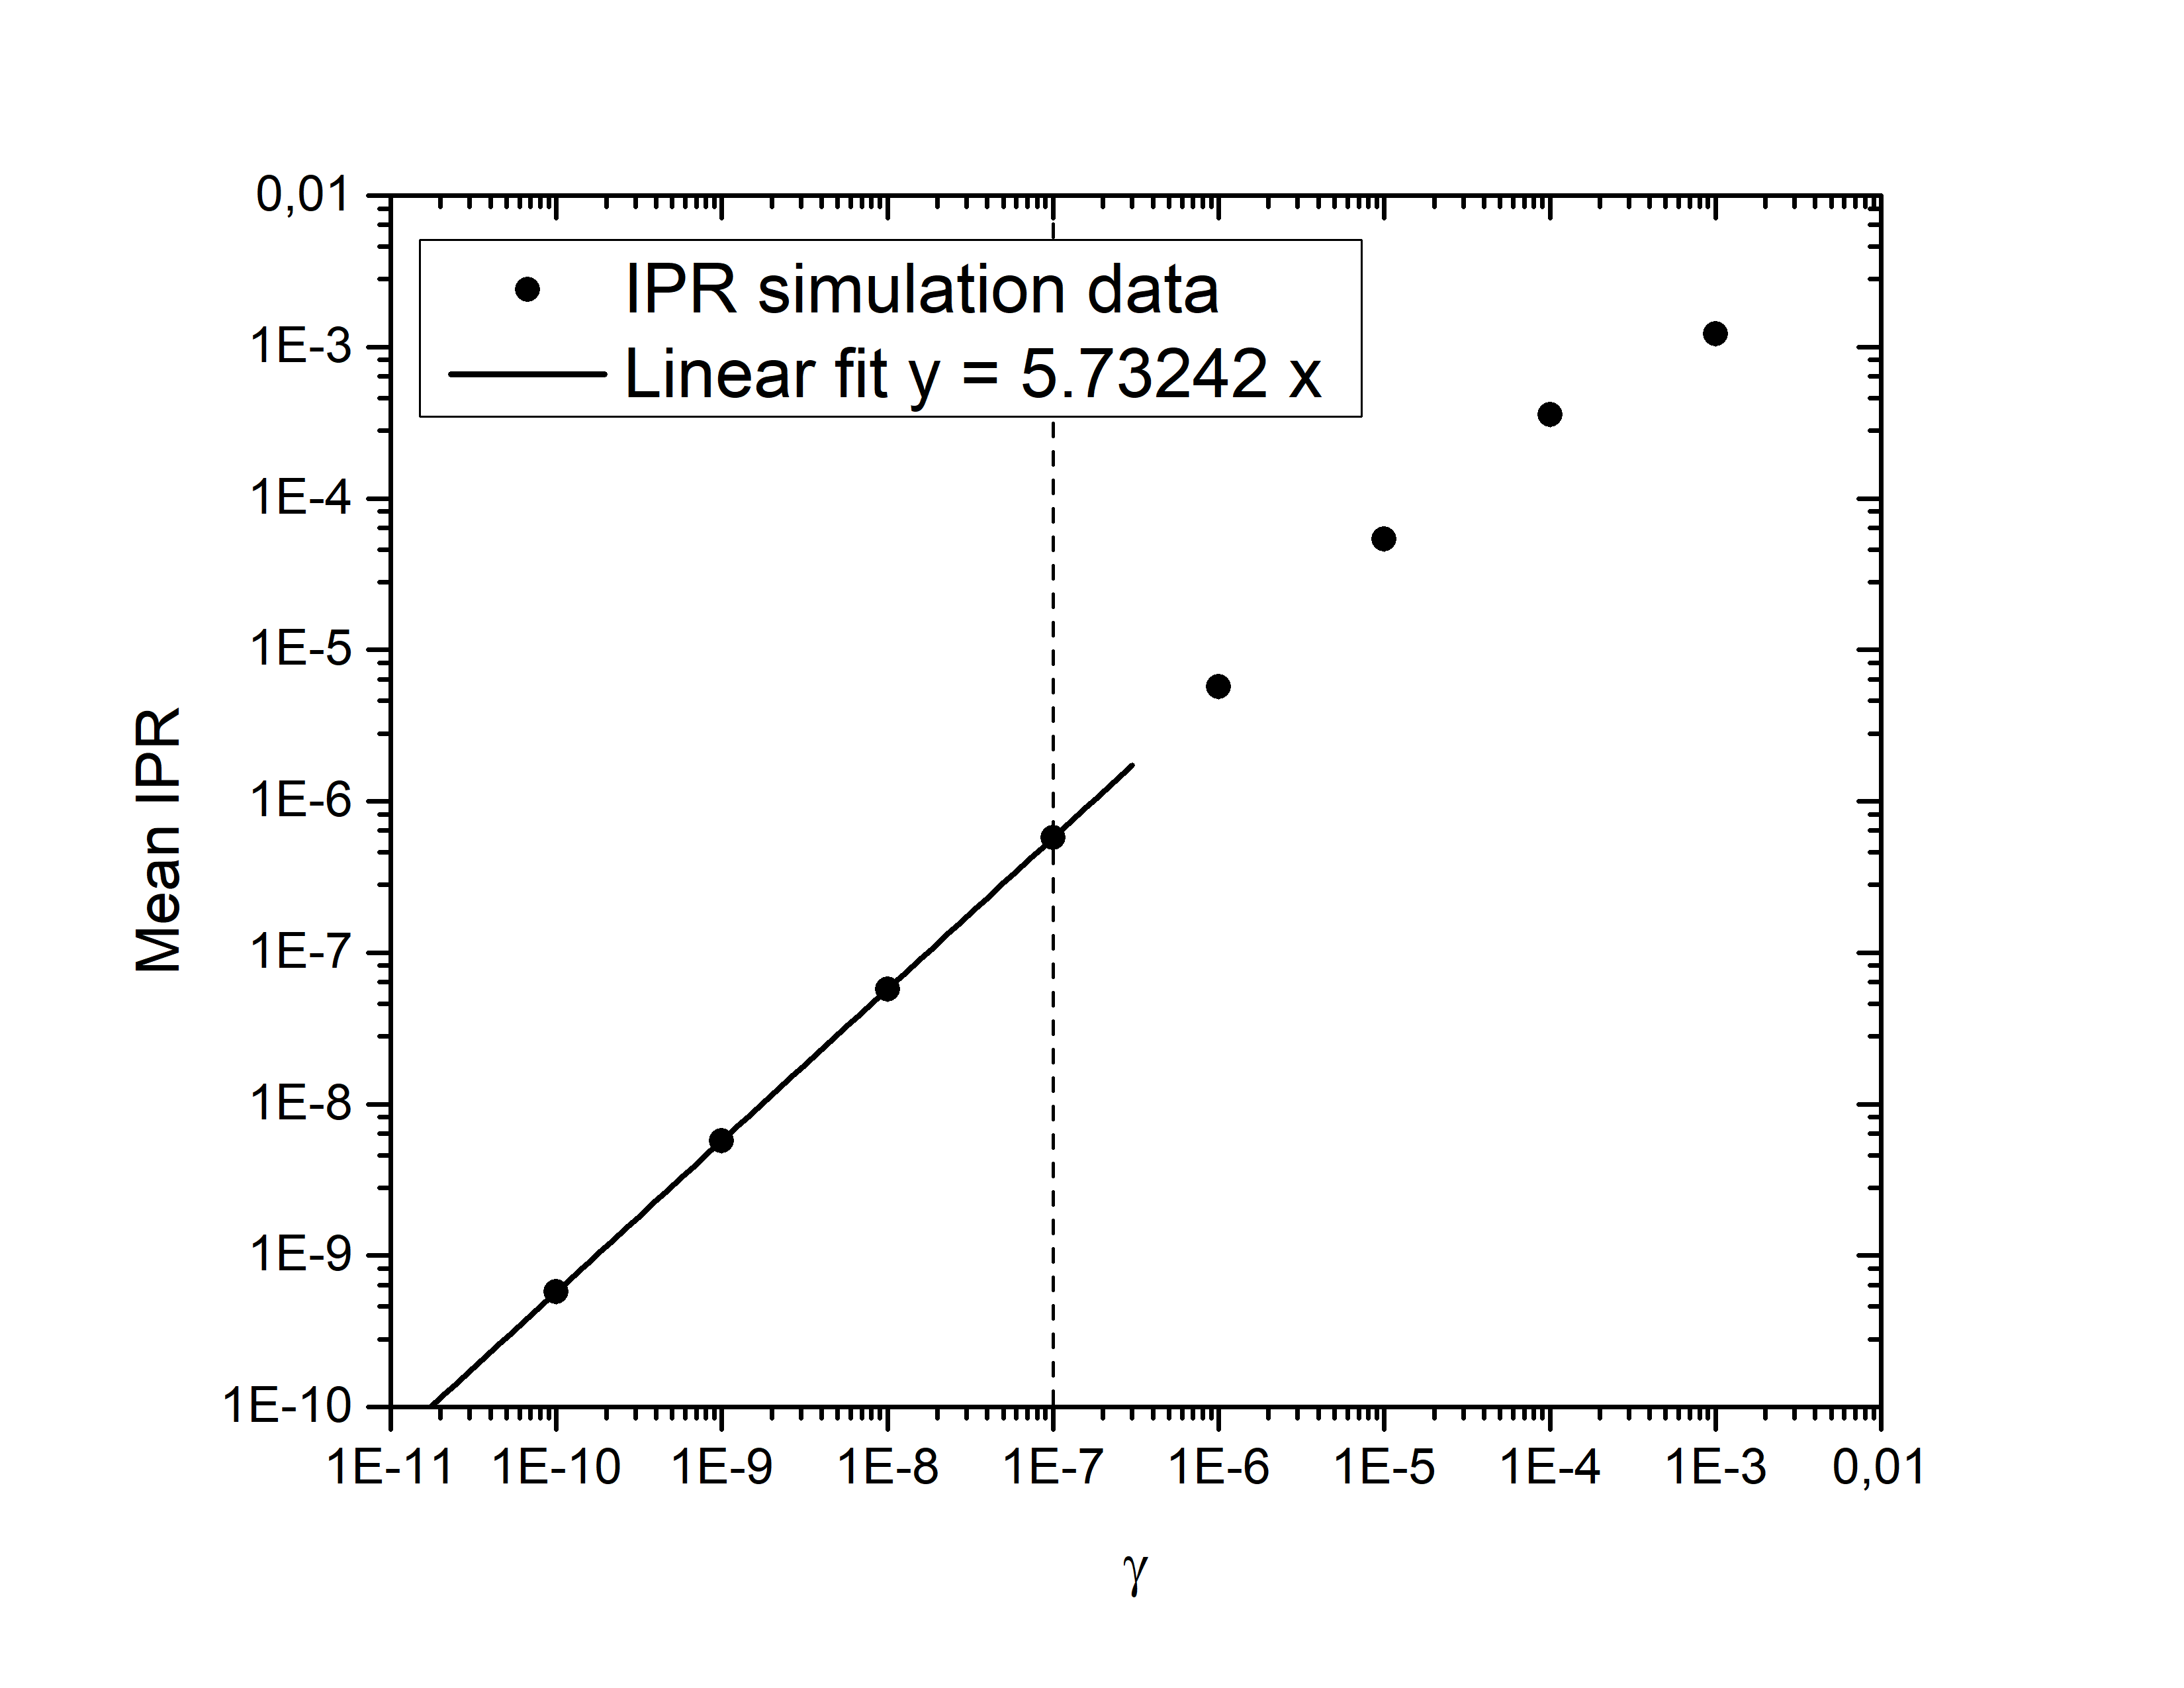
\includegraphics[width=0.49\textwidth]{Mean_IPR_gamma_dependence.png}
	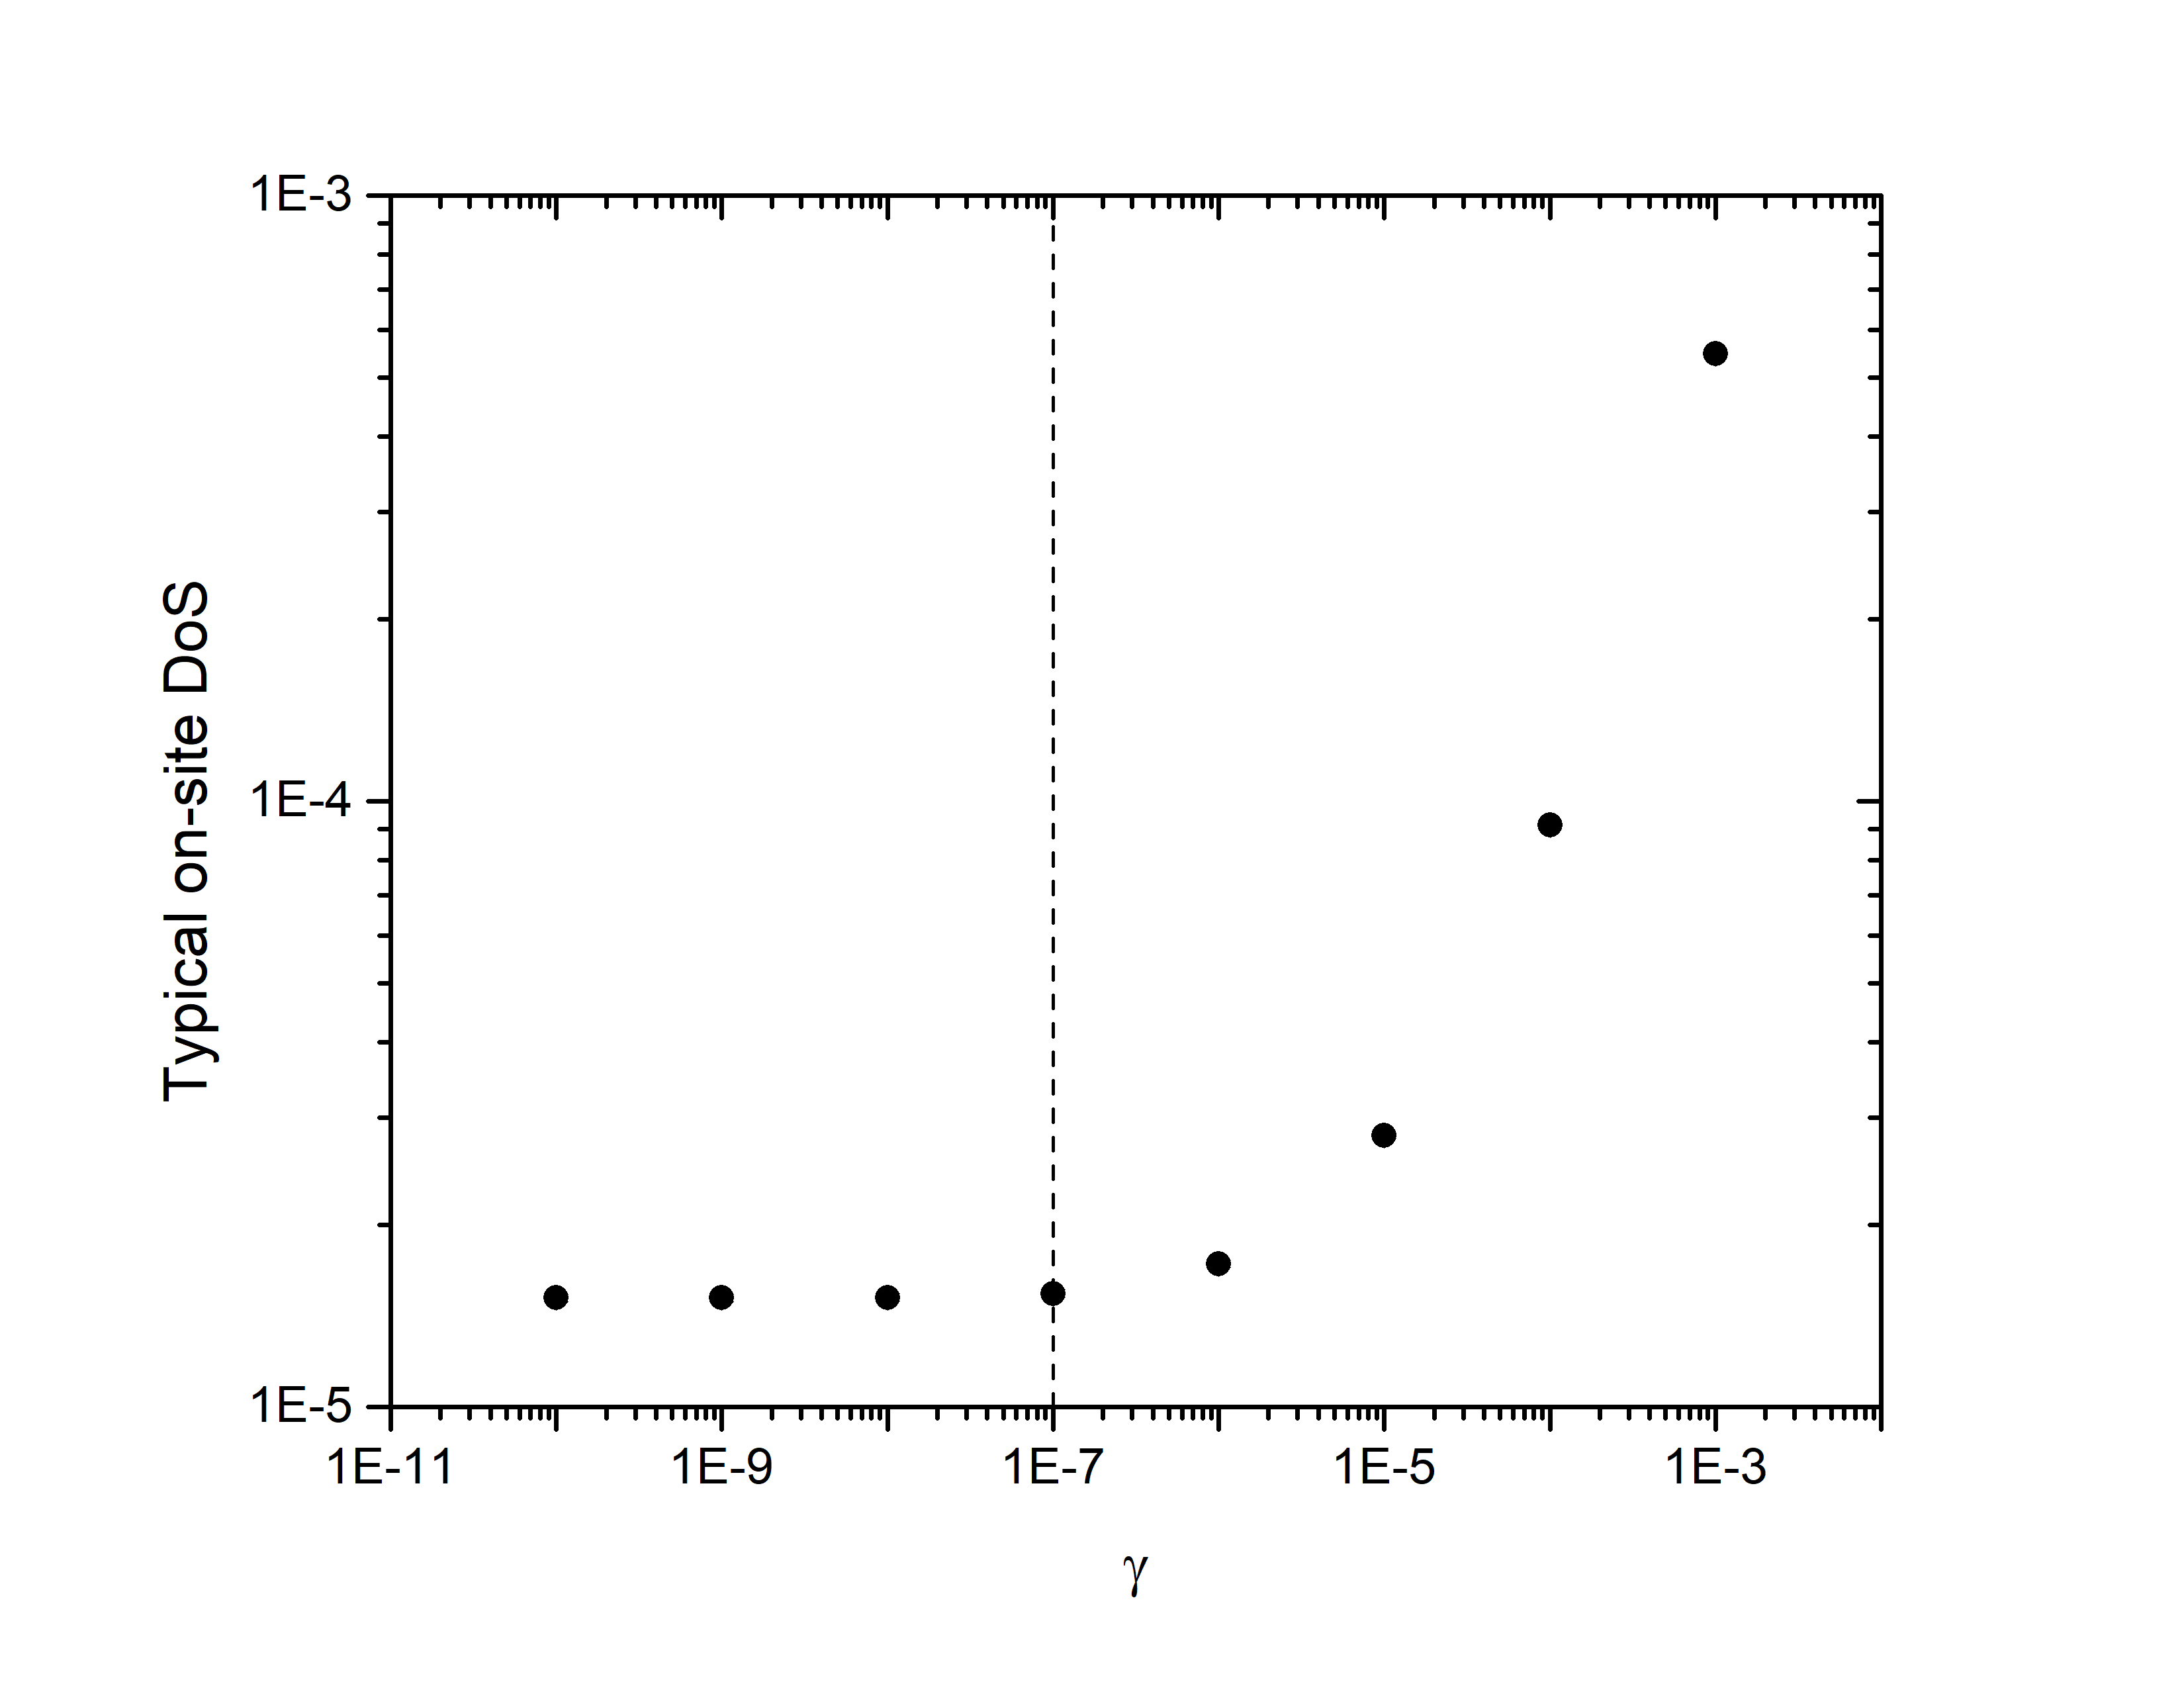
\includegraphics[width=0.49\textwidth]{Typical_DOS_gamma_dependence_for_IPR.png}
	\caption{Зависимость средней IPR (слева) и типичной плотности состояний (справа) от регуляризующего параметра $\gamma$. На обоих зависимостях пунктирной линией отмечено значение $\gamma$ насыщения типичной плотности состояний. Зависимость средней IPR от $\gamma$ сопровождается также графиков линейной аппроксимации в зоне насыщения. Параметры симуляции: $K = 30, M = 2^{25} \approx 3.4 \cdot 10^{8}$.}
\end{figure}



\section{Распределение мнимой части модельной функции Грина}
Рассмотрим далее уже не раз упоминавшуюся форму распределения плотности состояний. К обсуждению предлагается пример на Рис. \ref{fig:DOS_distribution_example} со следующими параметрами:
\begin{itemize}
	\item физические параметры $K = 15, g = 0.15, \Delta = 2 \exp\left\{ -\frac{1}{g} \right\}$;
	\item параметры алгоритма $M = 2^{25} \approx 3.4 \cdot 10^{8}, \gamma = 10^{-10}$.
\end{itemize}
Отметим, что в целом больших различий в качественных характеристиках этой формы при различных $K$ замечено не было, поэтому все важные особенности могут быть продемонстрированы на приведённом Рис. \ref{fig:DOS_distribution_example}. Также это означает, что показательным являются зависимости численных характеристик этого распределения, которые будут активно обсуждаться далее. 

\begin{figure}[h!]
	\label{fig:DOS_distribution_example}
	\centering
	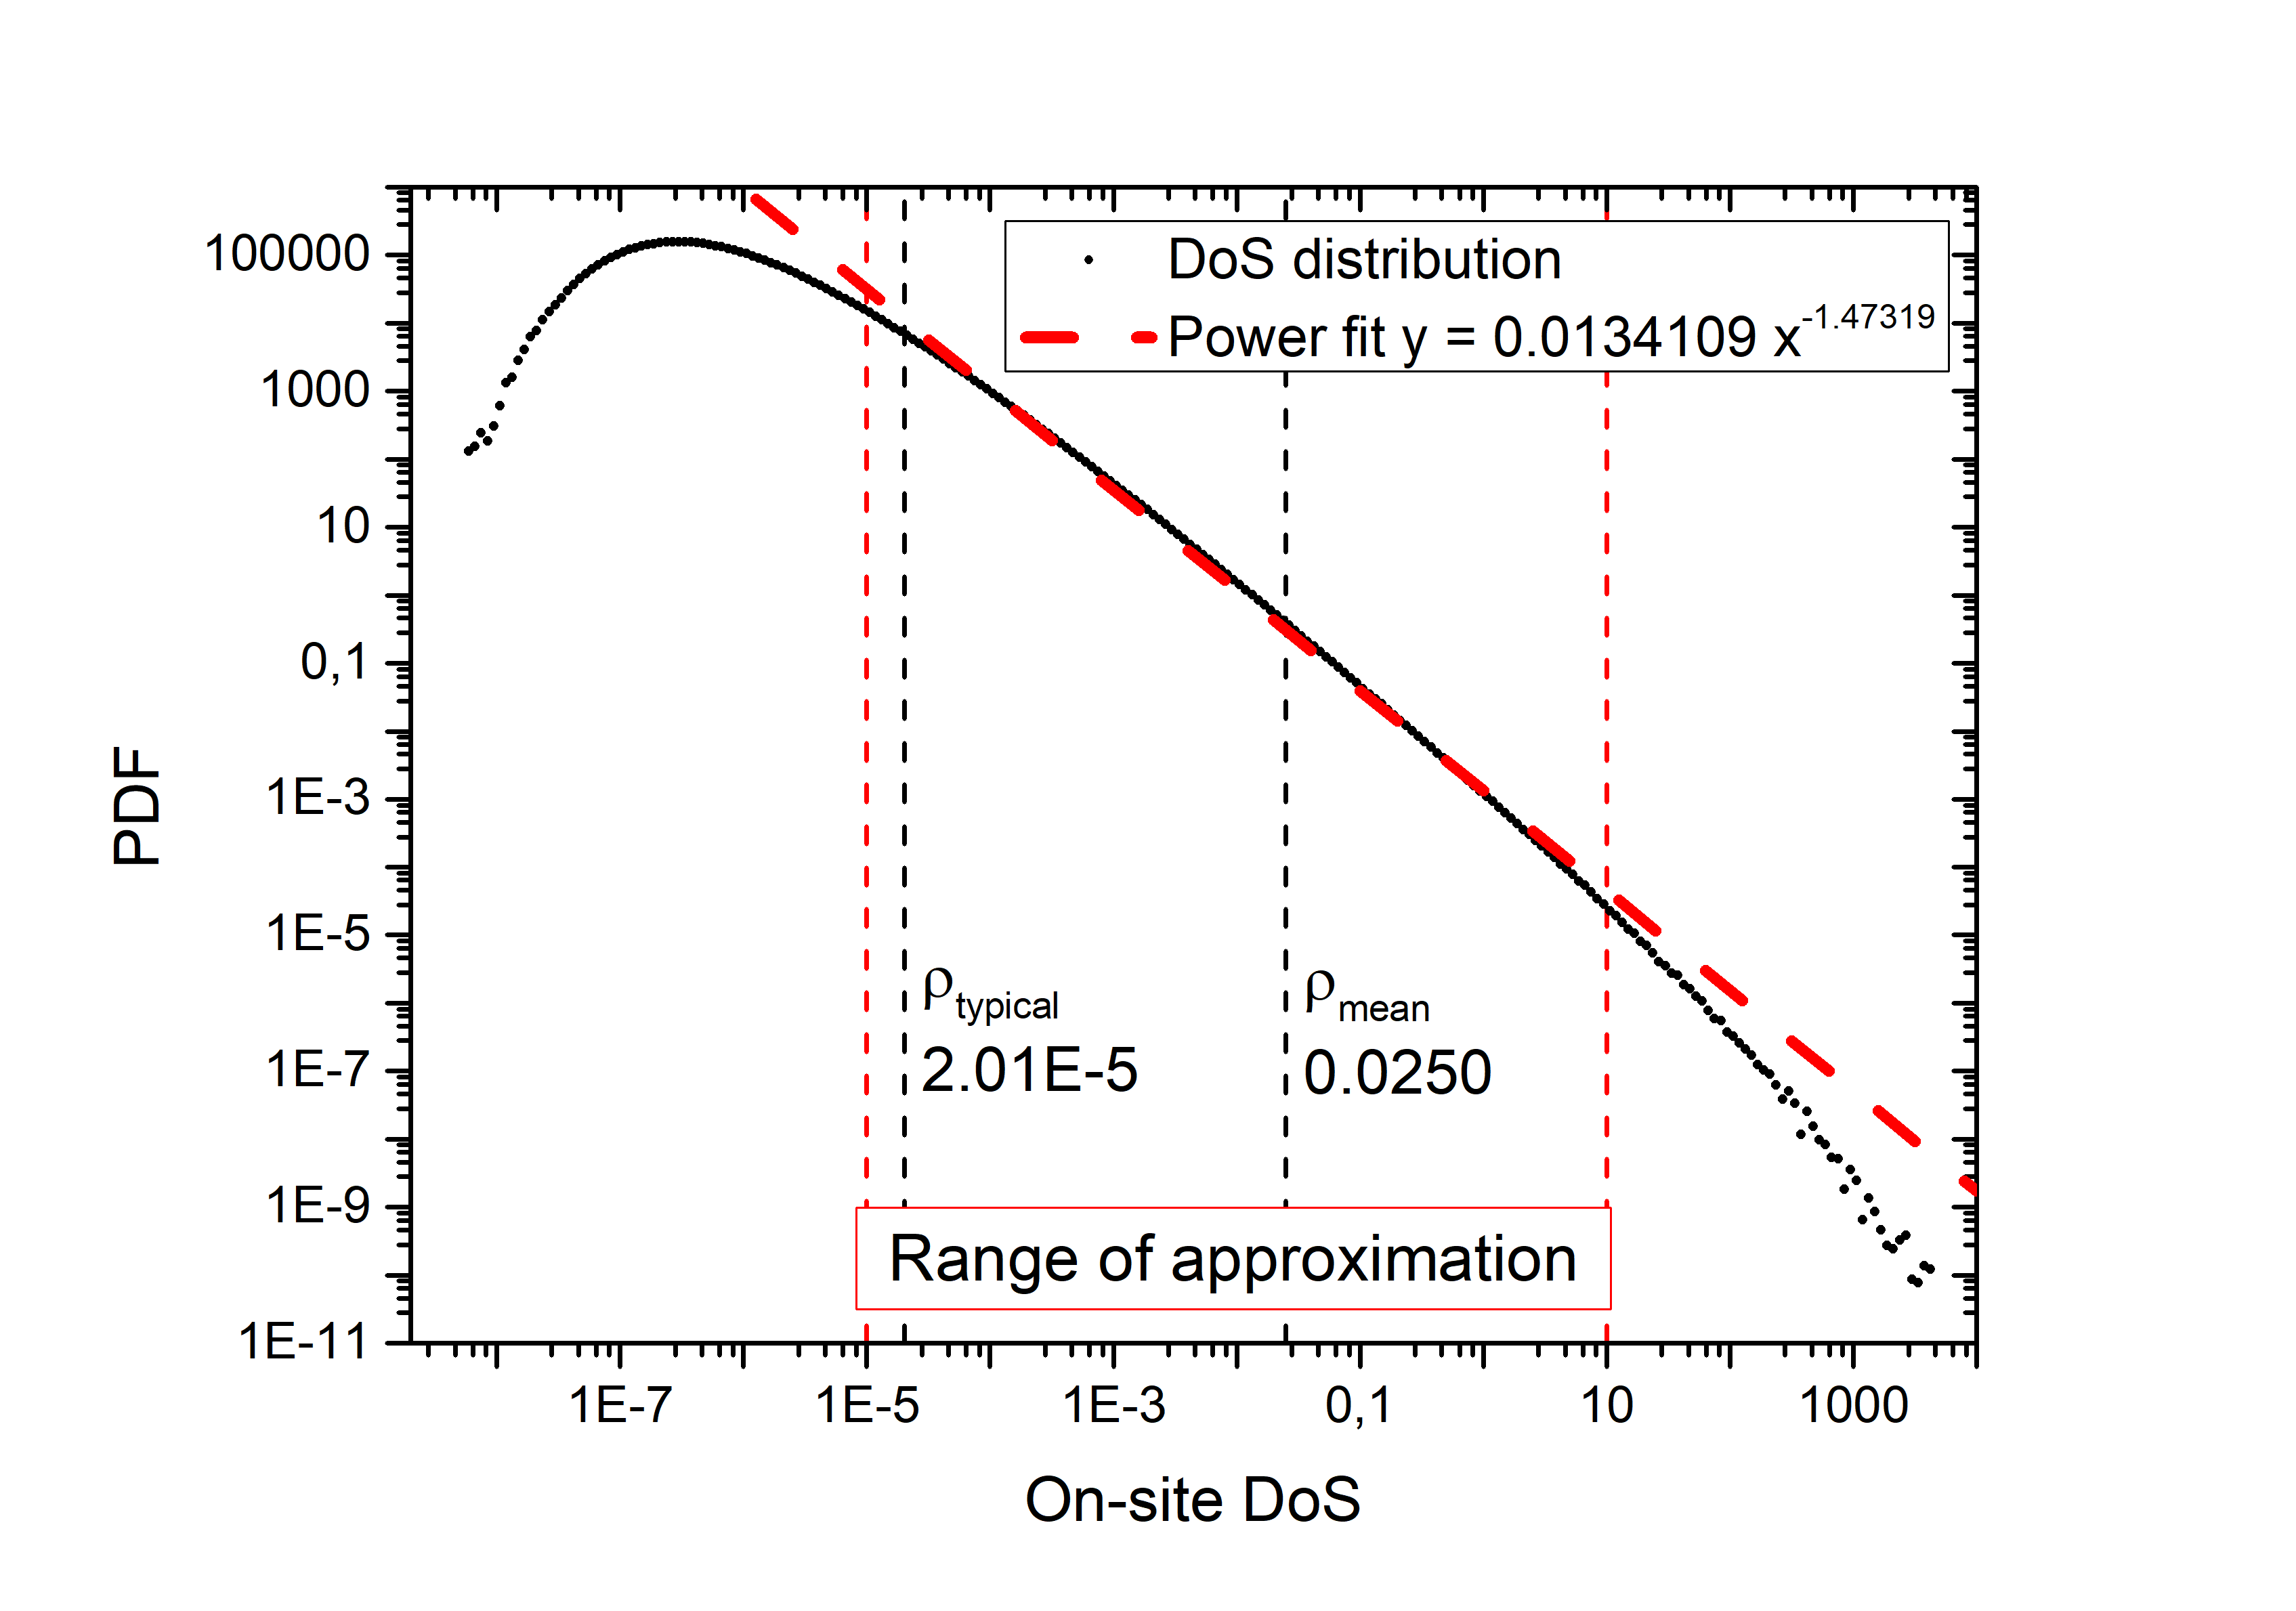
\includegraphics[width=0.9\textwidth]{DOS_distribution_example.png}
	\caption{Распределение локальной плотности состояний. Параметры см. в тексте. На графике также изображена степенная аппроксимация секции распределения, ограниченная красными пунктирными линиями. Вид зависимости для аппроксимации также указан на графике. Чёрными пунктирными линиями показаны характеристики распределения -- средняя и типичная плотность состояний с соответствующими численными значениями.}
\end{figure}

Зафиксируем наблюдаемые особенности распределения и следствия из них. Ещё раз подчеркнём, что эти особенности наблюдаются \textit{во всём диапазоне значений параметра $K$}:
\begin{enumerate}
	\item прежде всего, заметим, что в широких пределах поведение распределения является степенным, причём аппроксимация показывает значение показателя, близкое к $3/2$, т. е. распределение имеет <<длинный хвост>>.
	\begin{itemize}
		\item Важно заметить ещё одно обстоятельство, связанное с уже упомянутым соотношением рассматриваемой задачи с задачей Андерсона с диагональным беспорядком: наблюдаемый показатель степени очень близок к критическому показателю, наблюдаемым ровно на пороге локализации \cite{AAT}. Как мы продемонстрируем несколько позже, данное совпадение не случайно.
	\end{itemize}
	\item Степенное поведение реализуется в очень широких пределах: диапазон составляет минимум 6 порядков.
	\item Среднее $\langle \rho \rangle \approx 2.5 \cdot 10^{-2}$ и типичное $\exp \langle \ln \rho \rangle  \approx 2.5 \cdot 10^{-2}$  для данного распределения отличаются на три порядка. Данное поведение легко понять на основе уже упомянутого степенного поведения распределения:
	\begin{itemize}
		\item само распределение в широких пределах $\rho_{min} \ll \rho \ll \rho_{max}$ имеет степенной вид, из чего можно оценить его нормировку:
		$$
		P(x) \sim A x^{-3/2} \Rightarrow A \sim \left[ \int \limits_{ \rho_{min} }^{ \rho_{max} } \frac{dx}{x^{3/2}} \right]^{-1} \sim \frac{1}{2} \sqrt{\rho_{min}}
		$$
		Эта нормировка выходит чувствительной к нижней отсечке распределения, которая является наиболее часто выпадающей. По порядку полученная оценка хорошо описывает наблюдаемое поведение: $\frac{1}{2} \sqrt{ \rho_{min} } \sim 2 \cdot 10^{-3}$, что неплохо соотносится с результатами аппроксимации.
		\item В таком распределении среднее значение оценивается как
		$$
		\langle \rho \rangle \sim \int \limits_{ \rho_{min} }^{ \rho_{max} } \frac{A dx}{x^{1/2}} \sim 2 A \sqrt{\rho_{max}} \sim \sqrt{\rho_{max} \rho_{min}} 
		$$
		Результат показывает, что среднее набирается на экстремальных значениях распределения: частота выпадения больших значений довольно мала, и тем не менее, их обрезка явно входит в ответ. Данная формула находит отражение на \ref{fig:DOS_distribution_example}: в логарифмическом масштабе среднее находится примерно посредине между границами степенной зависимости, в соответствии с полученной оценкой. 
		\begin{itemize}
			\item Полученная оценка объясняет уже отмеченные ранее в \autoref{Numer} детали поведения этой величины в рамках численного счёта: при плохом выборе $\gamma, M$ обрезки диктуются не свойствами системы, а этими параметрами внутренними параметрами. При этом нижняя граница фиксированна величиной $\gamma$, а верхняя сильно флуктуирует из-за малого размера выборки, что приводит к появлению в динамике алгоритма уже описанных <<выбросов>>.
		\end{itemize}
		\item Для типичного подобные рассуждения приводят к уже анонсированному ранее результату
		$$
		\rho_{typ} \sim \exp\left\{ \int \limits_{ \rho_{min} }^{ \rho_{max} } \frac{A dx}{x^{3/2}} \ln x \right\} \sim \exp\left\{ 2 A \left( 2 + \ln \rho_{min} \right) \frac{1}{ \sqrt{\rho_{min}} } \right\} \sim \rho_{min}
		$$
		Такие оценки демонстрируют, что в отличие от среднего, типичное, как и нормировка распределения, набирается на малых значениях $\rho$, что можно усмотреть и на Рис. \ref{fig:DOS_distribution_example}: типичное по значению близко к границе степенного поведения.
		\item Можно оценить различие среднего и типичного:
		$$ \frac{ \langle \rho \rangle }{ \rho_{typ} } \sim \sqrt{\frac{ \rho_{max} }{ \rho_{min} }} $$
		Для видимого отношения обрезок $\sim 10^6$ получаем наблюдаемое отношение среднего и типичного $\sim 10^3$.
	\end{itemize}
\end{enumerate}



\section{Зависимость физических величин от параметра $K$}
Наконец, мы подошли к главному количественному результату нашей работы: в этом разделе мы приведём зависимости средней и типичной плотности состояний от $K$, и на основании этих зависимостей построим фазовую диаграмму для исследуемой модели. Неизменные параметры всё те же: $g = 0.15, \Delta = 2 \exp \left\{ -\frac{1}{g} \right\}$.


\subsection{Зависимости от параметра $K$}

\begin{figure}[h!]
	\label{fig:Mean_DOS_dependence_from_K}
	\centering
	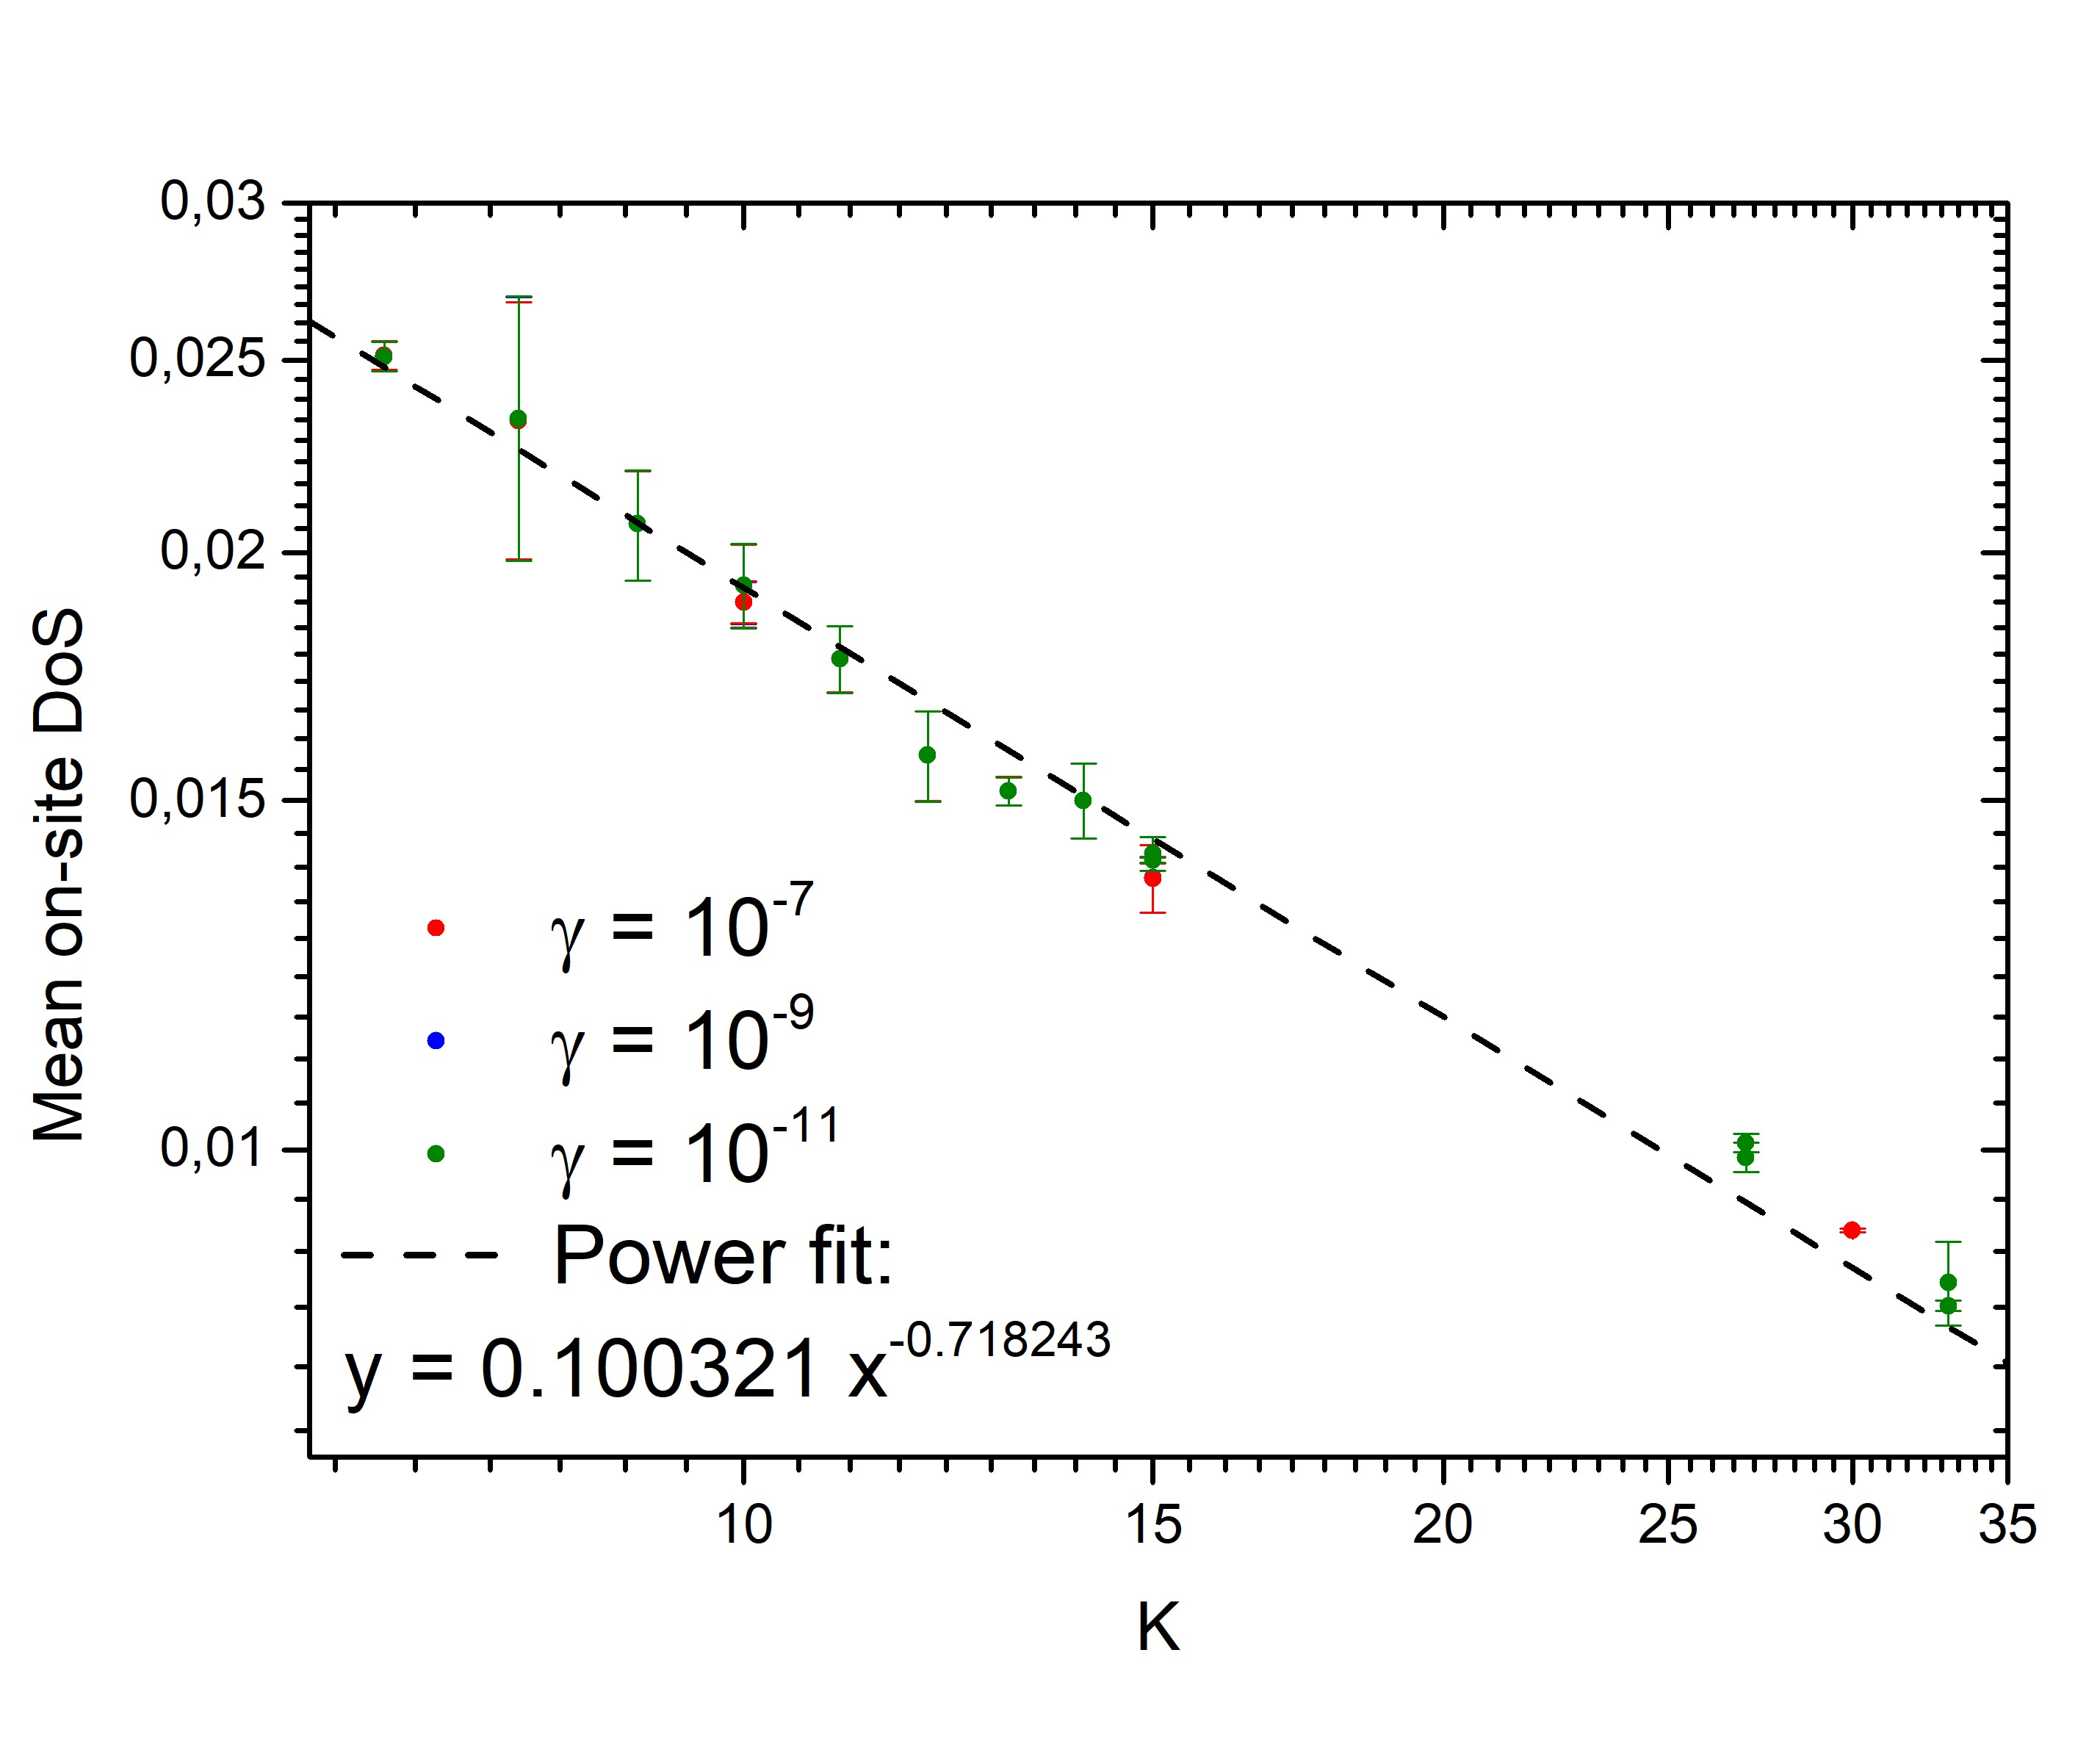
\includegraphics[width=0.49\textwidth]{Mean_DOS_dependence_K_small.jpg}
	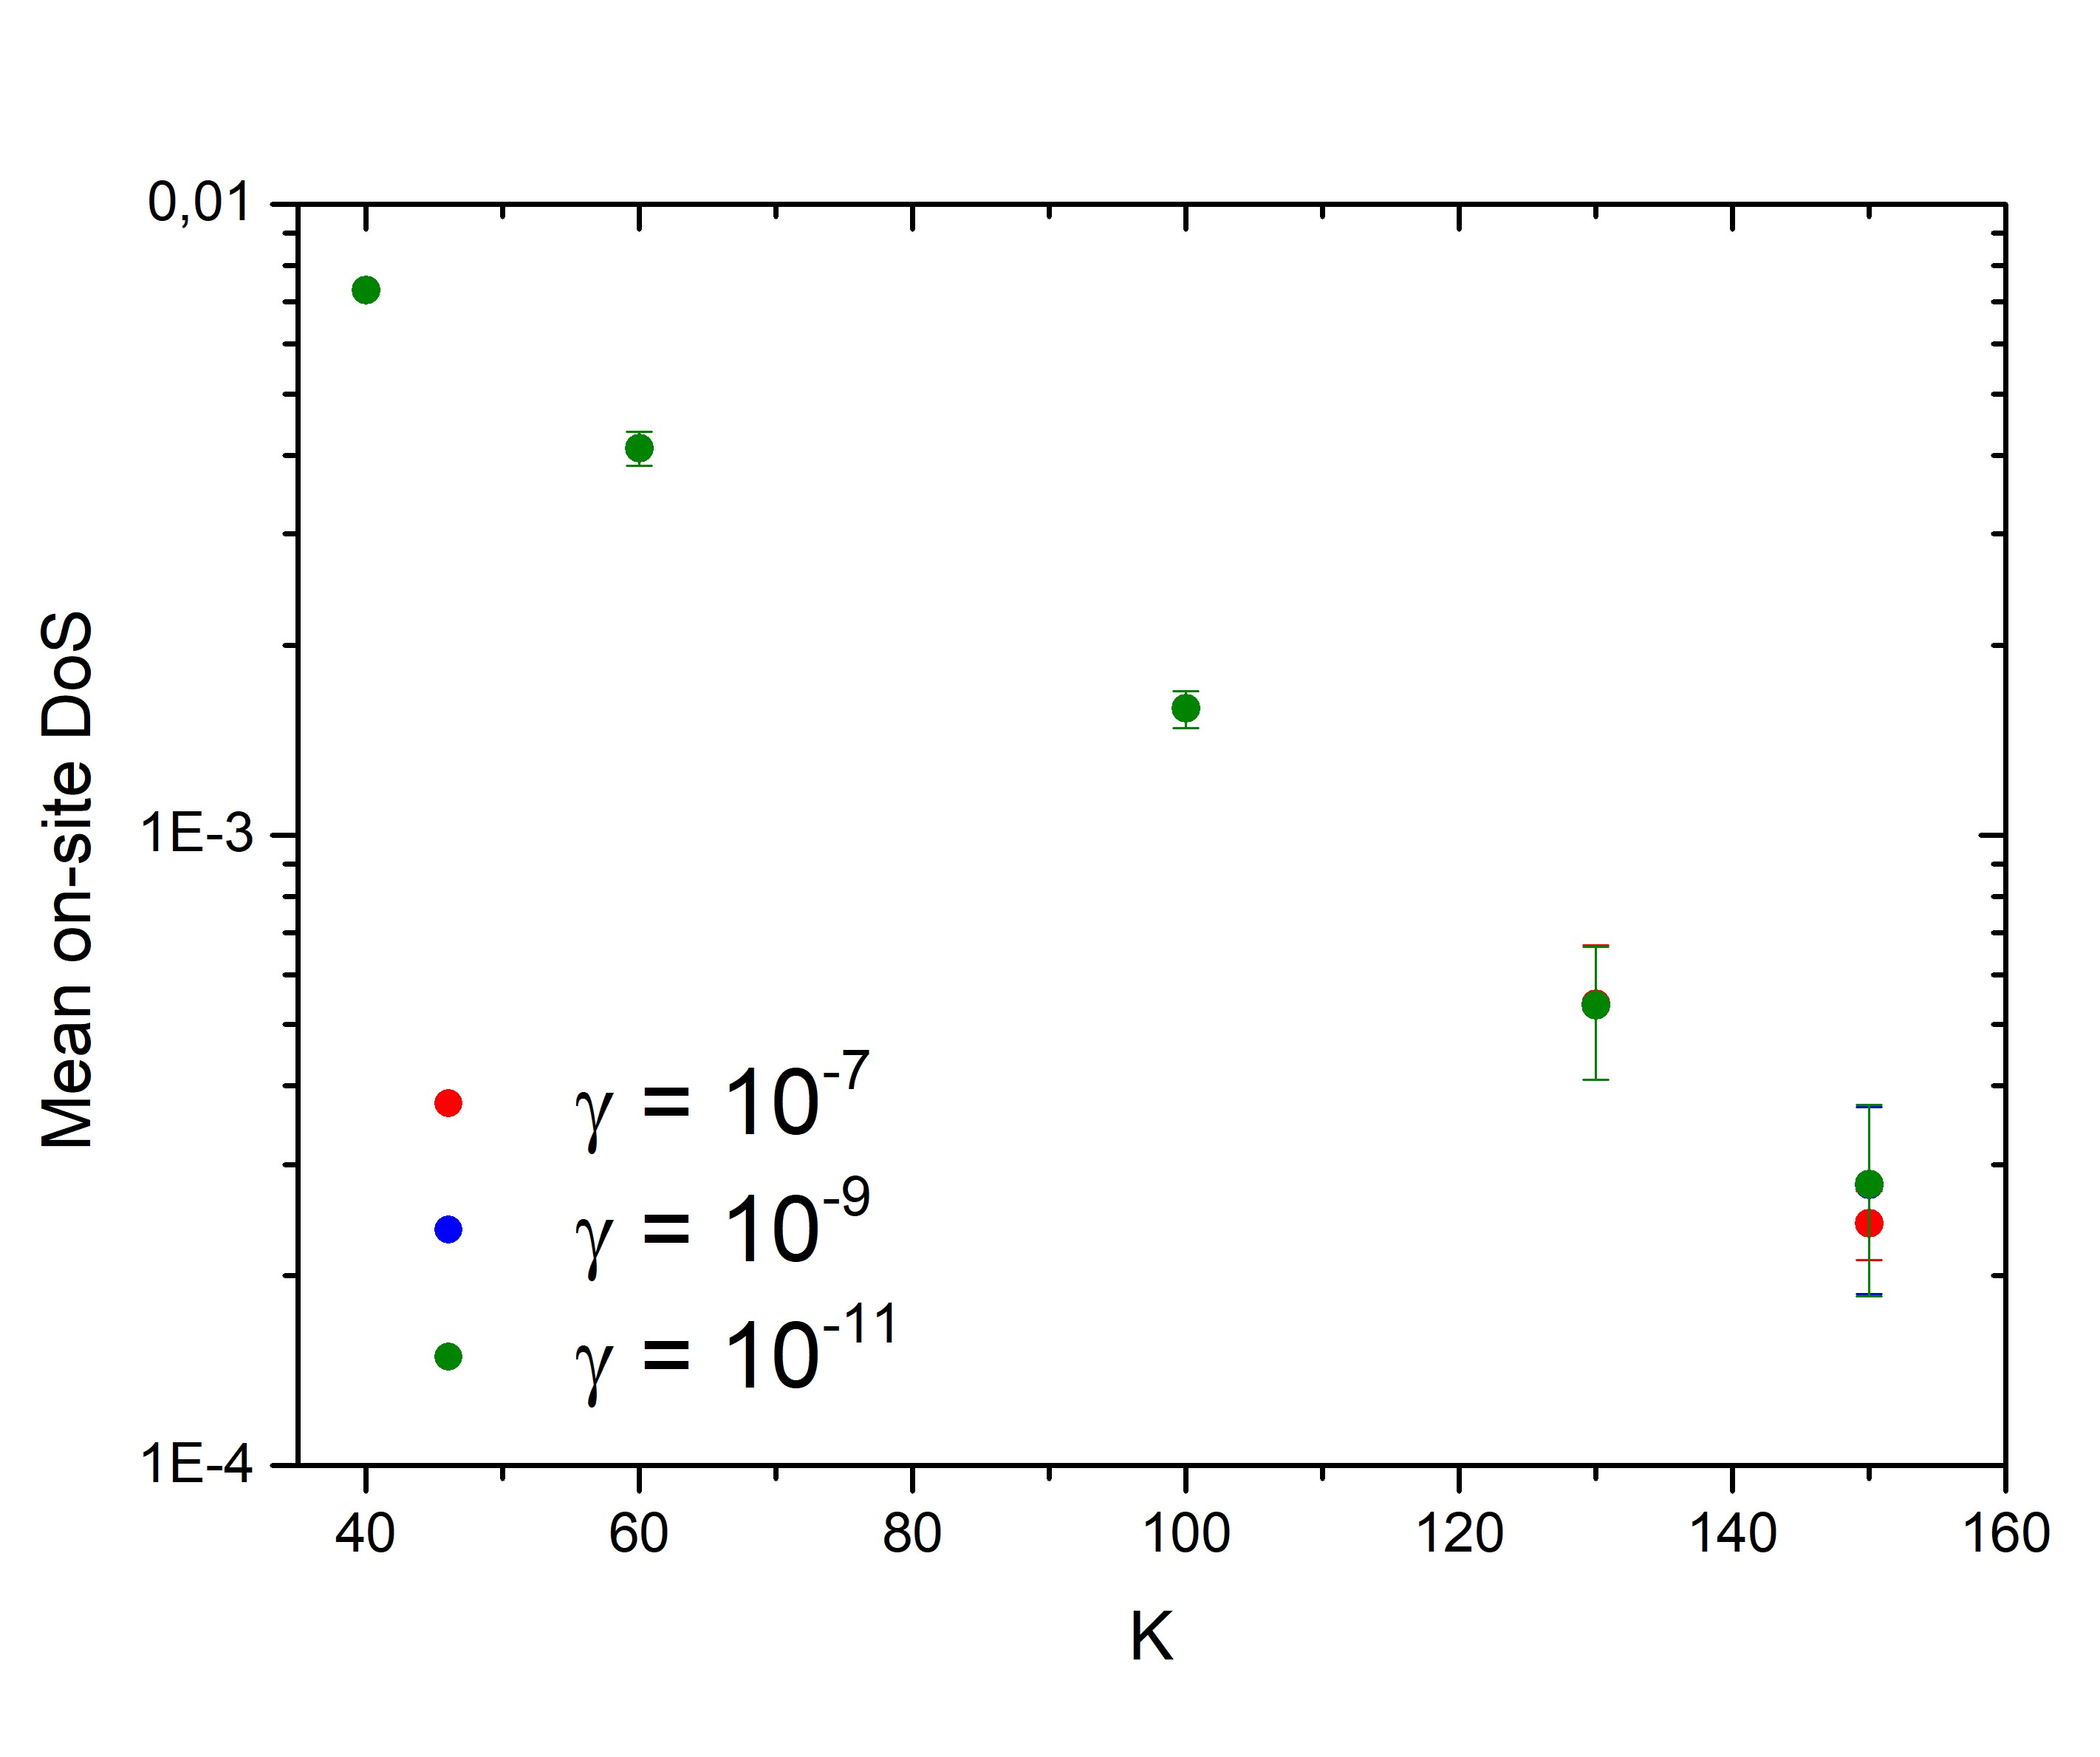
\includegraphics[width=0.49\textwidth]{Mean_DOS_dependence_K_large.jpg}
	\caption{Зависимость средней плотности состояний $\langle \rho \rangle$ от числа ветвления $K$. Данные разделены на две части, отображаемые в разных масштабах: малые $K < 35$ построены в масштабе $LogX, LogY$, а большие $K > 35$ --- $LinX, LogY$. На рисунке представлены версии зависимостей для трёх различных значений параметра $\gamma$. Наличие нескольких точек при данном значении $K, \gamma$ соответствует разным размерам выборки $M$. Область малых значений $K < 35$ также оснащена степенной аппроксимацией данных.}
\end{figure}

\begin{figure}[h!]
	\label{fig:Typical_DOS_dependence_from_K}
	\centering
	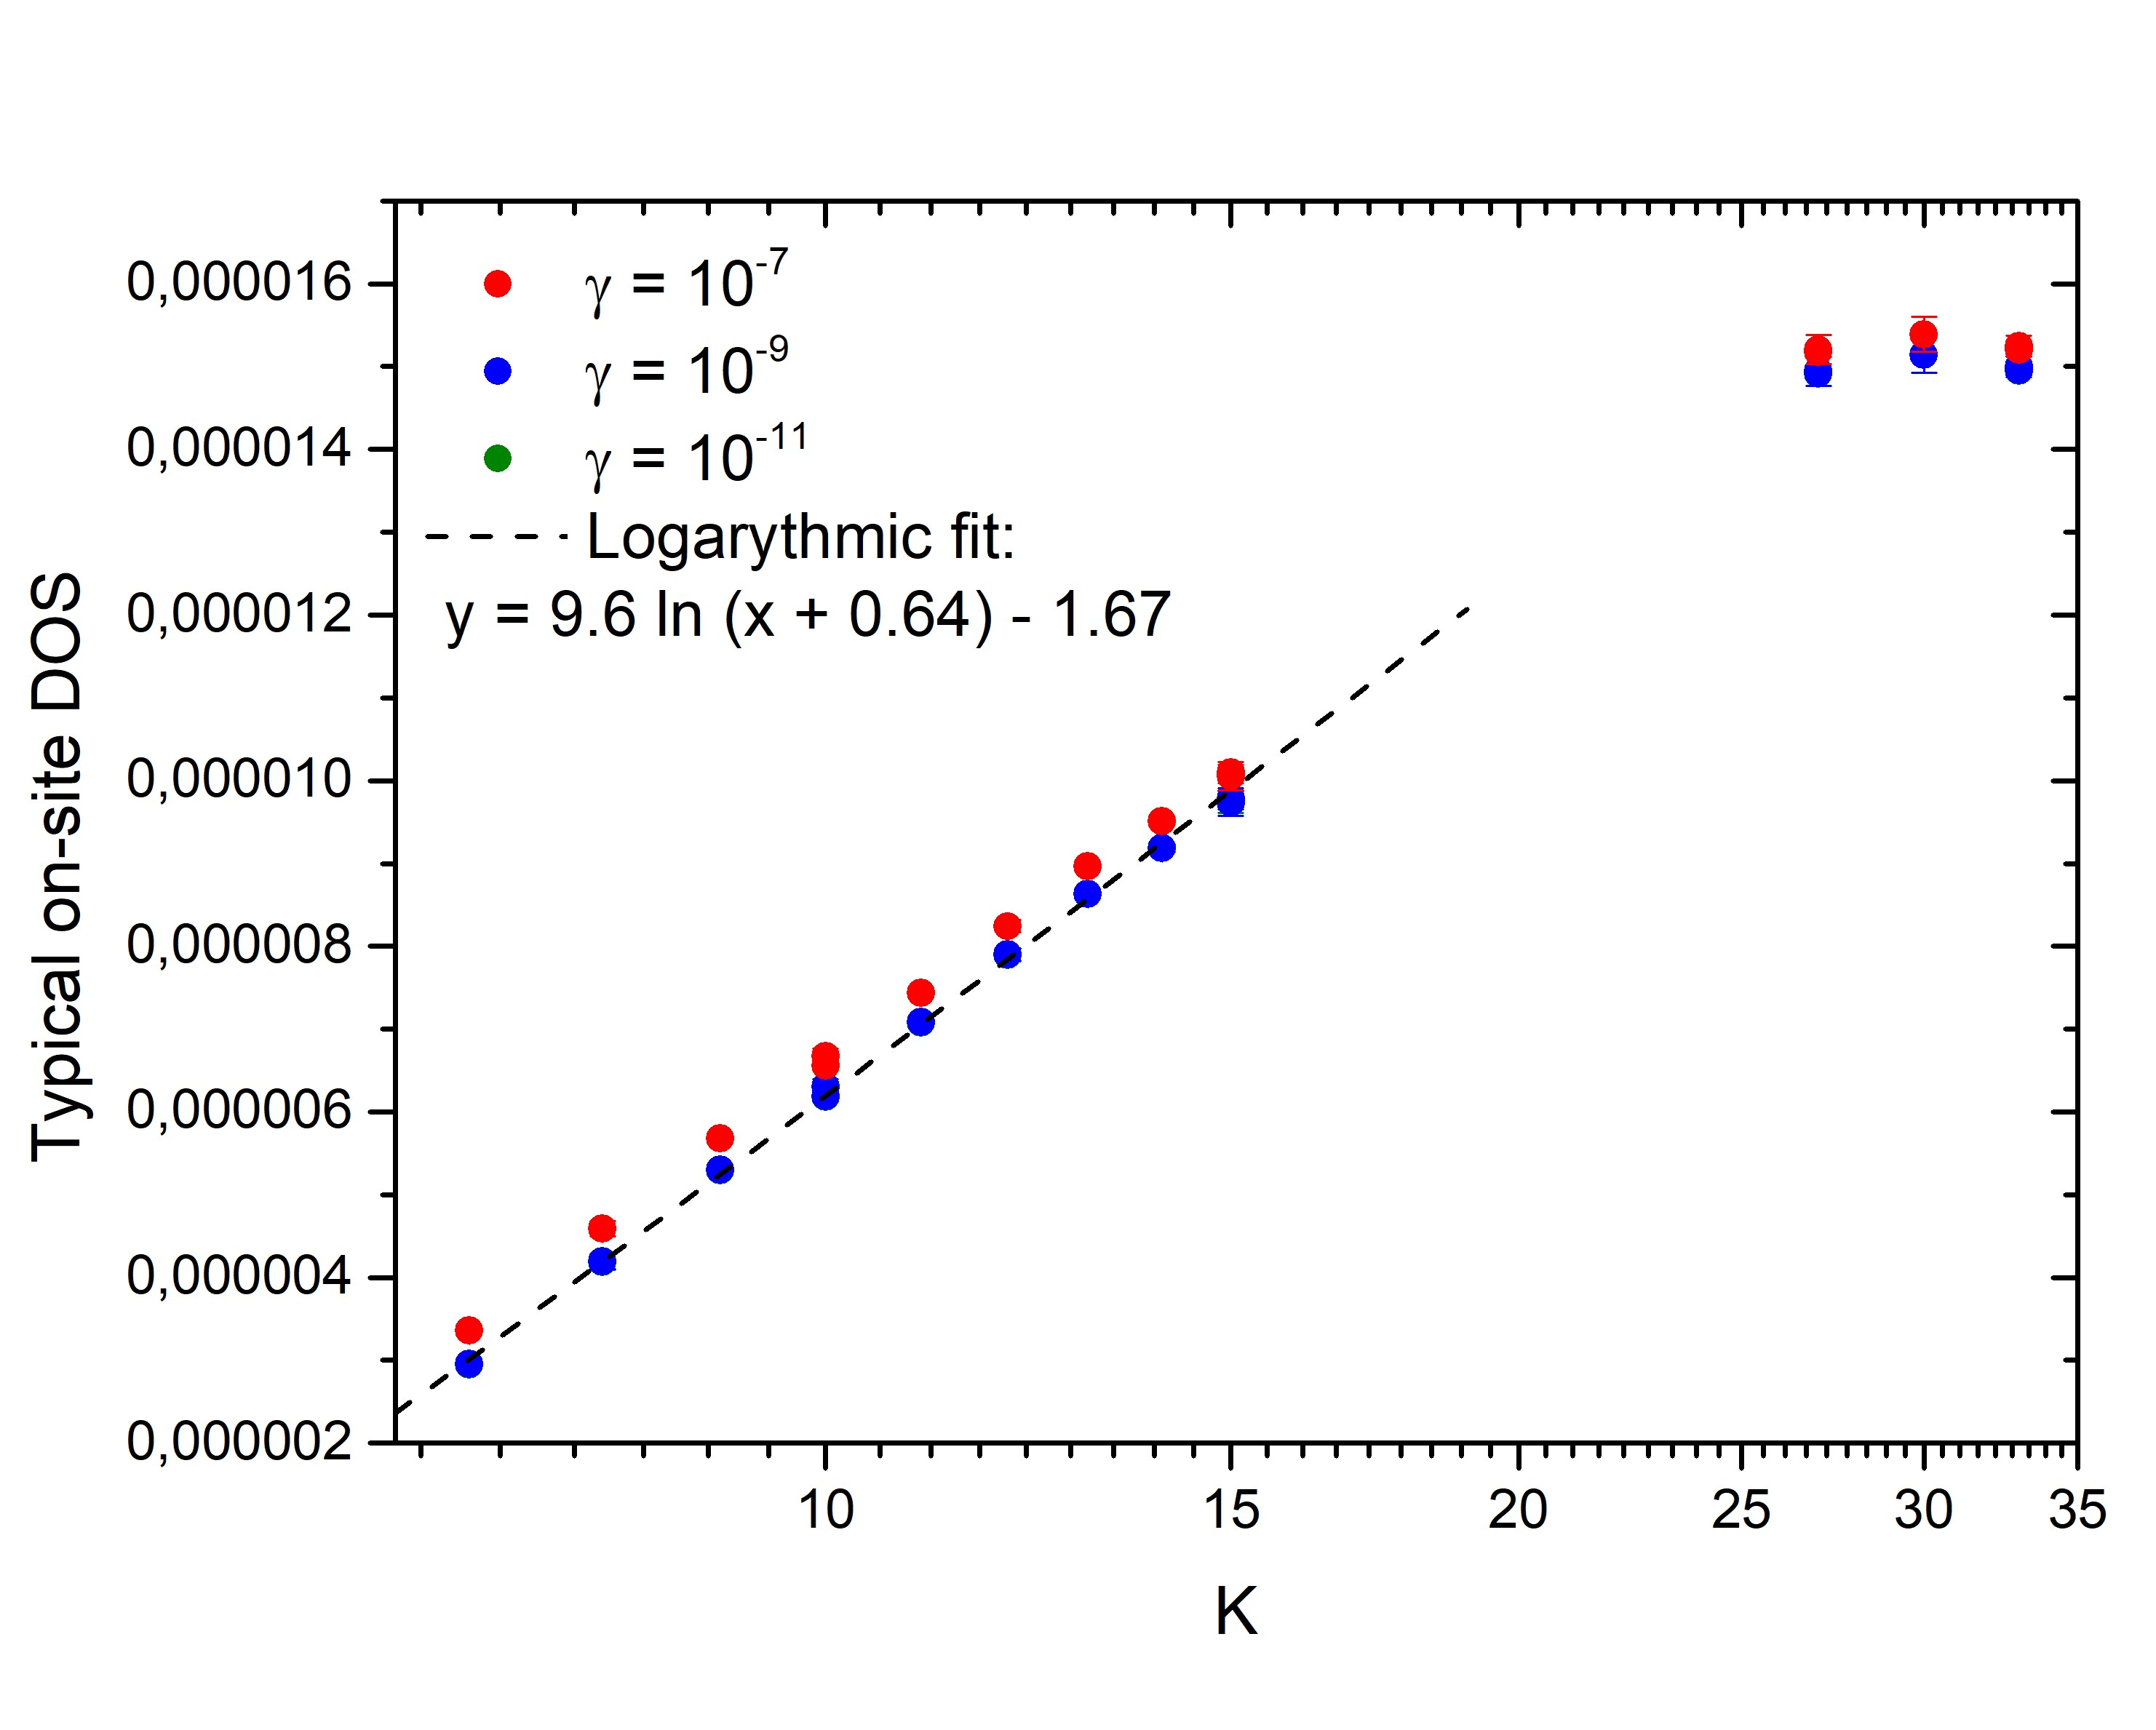
\includegraphics[width=0.49\textwidth]{Typical_DOS_dependence_K_small.jpg}
	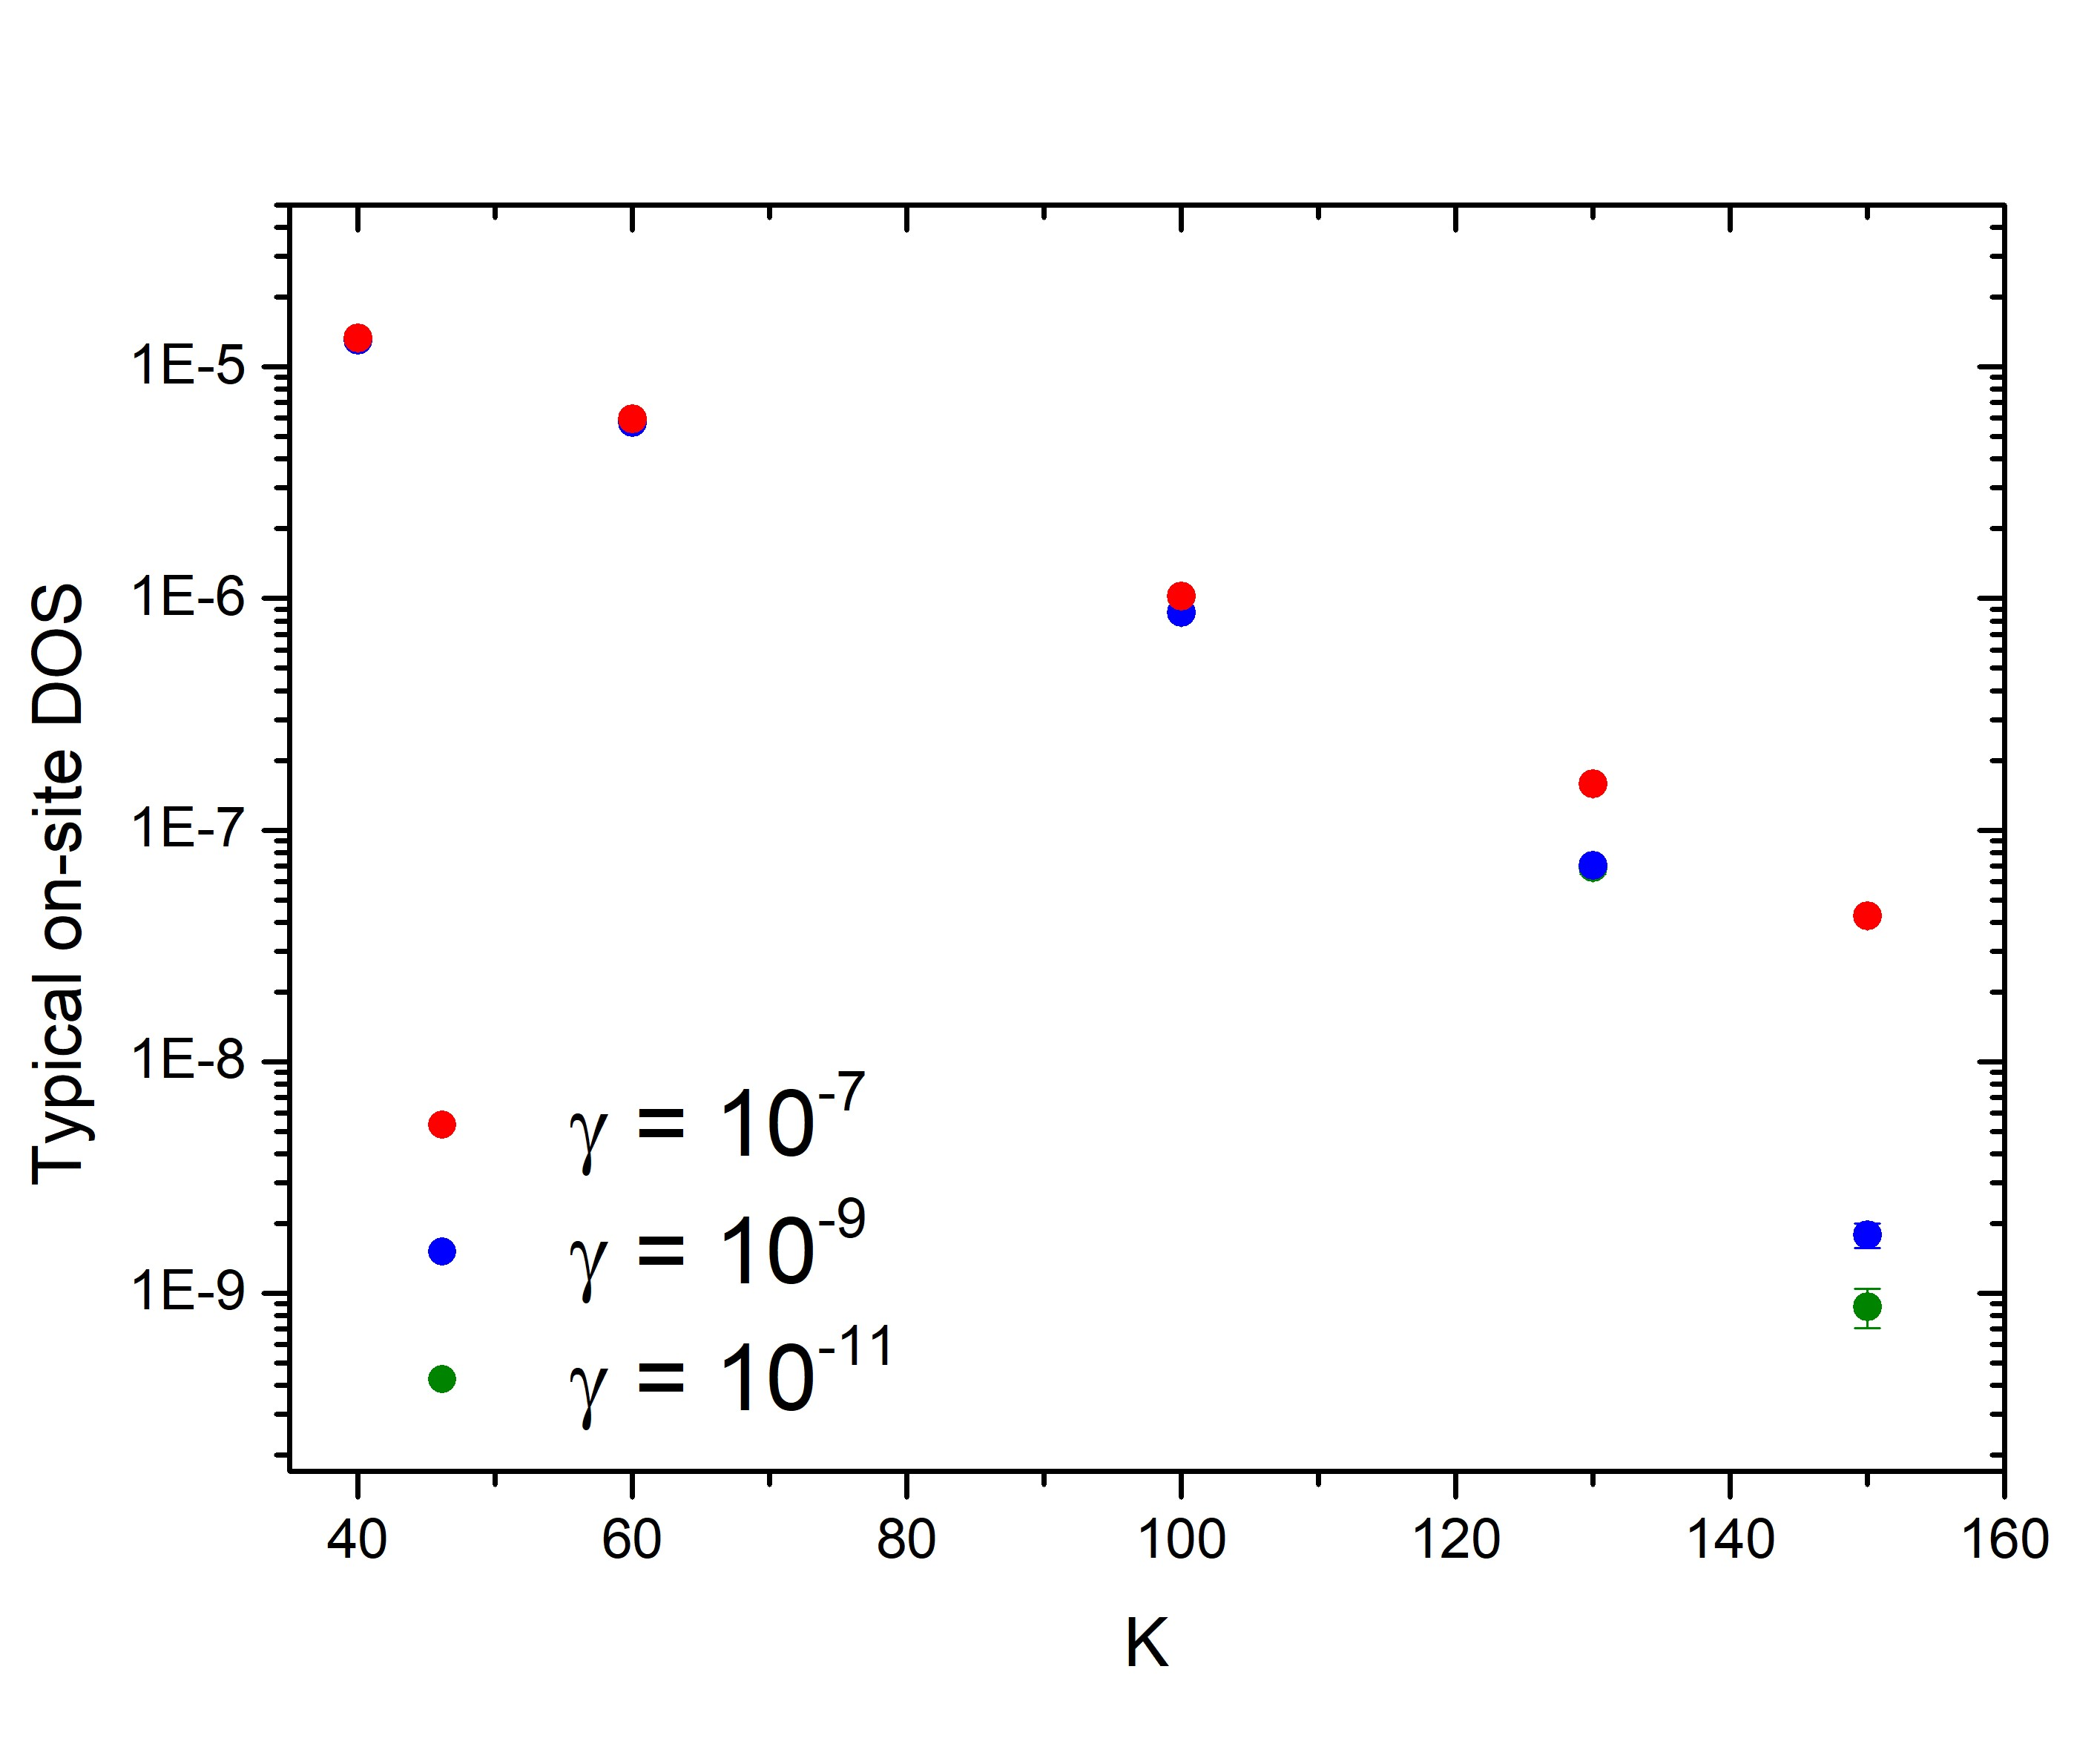
\includegraphics[width=0.49\textwidth]{Typical_DOS_dependence_K_large.jpg}
	\caption{Зависимость типичной плотности состояний $\exp \langle \ln \rho \rangle$ от числа ветвления $K$. Данные разделены на две части, отображаемые в разных масштабах: малые $K < 35$ построены в масштабе $LogX, LinY$, а большие $K > 35$ --- $LinX, LogY$. На рисунке представлены версии зависимостей для трёх различных значений параметра $\gamma$. Наличие нескольких точек при данном значении $K, \gamma$ соответствует разным размерам выборки $M$. Область малых значений $K < 35$ также оснащена логарифмической аппроксимацией части данных.}
\end{figure}

На Рис. \ref{fig:Mean_DOS_dependence_from_K} и \ref{fig:Typical_DOS_dependence_from_K}  представлены зависимости соответственно средней и типичной плотности состояний от числа ветвления $K$. Дадим ряд пояснений к интерпретации графиков:
\begin{itemize}
	\item Поскольку среднее значение, как мы уже отмечали ранее в \autoref{Numer}, является при некоторых значениях параметров сильно флуктуирующей величиной, то в этих случаях использовались данные стационарных итераций алгоритма популяционной динамики: среднее и его погрешность оценивались как, соответственно, среднее и дисперсия возникающего временного ряда. Видимое отсутствие погрешностей означает, что они меньше размера точки.
	\item Зависимости естественным образом разделены на две асимптотические области: малые $K < 35$ и большие $K > 35$. Обратим внимание на то, что в разных областях выбран разный масштаб осей для иллюстрации соответствующей асимптотики (см. подписи к рисункам). Для малых $K$ эти асимптотики явно продемонстрированы аппроксимациями. При больших $K$ данных для достоверных утверждений недостаточно.
	\item На всех картинках представлены версии зависимостей для разных значений параметра $\gamma$, что позволяет судить о степени достоверности данных. Отсутствие точек соответствующего цвета означает совпадение значений.
	\item Наличие нескольких точек с одинаковыми значениями $K, \gamma$ отображает различные размеры выборки $M$ (что, как мы проиллюстрировали в \autoref{Numer}, влияет на погрешность и значение средней плотности). Эти данные также призваны более полно отобразить степень однозначности интерпретации данных.
	\item Данные для $K \le 6$ и $K \ge 160$ не приводятся, поскольку являются недостоверными в указанном выше смысле.
\end{itemize}

Основные наблюдения касательно этих результатов следующие:
\begin{enumerate}
	\item во-первых, крайне любопытным выглядит появившаяся характерная точка $K = 35$, разделяющая набор данных на две части с абсолютно разным поведением. Физической интерпретации у этой точки на данный момент нет. Потенциальным кандидатом выглядит близко расположенная точка $K_2 \approx 30$, однако, согласно её определению, она имеет другой физический смысл. Чтобы проверить правдивость этой гипотезы, необходимо исследовать данные при других значениях констант $g$, и если эта точка будет ярко выражена --- изучить зависимость её положения от $g$ и сравнить с формулой \eqref{eq:K2_definition}. К сожалению, очевидный колоссальный объём для выполнения этой программы не выглядит выполнимым за разумное время.
	\item Обратимся к части данных с малыми $K < 35$. Здесь мы можем наблюдать следующие вещи:
	\begin{itemize}
		\item В целом здесь мы наблюдаем сравнительно слабые в смысле масштаба относительных изменений зависимости. Однако, они имеют хорошо выраженный вид, что отражено соответствующими аппроксимациями.
		\item Точка $K = 35$ характеризует для обоих зависимостью точку окончания асимптотики: график для среднего имеет в этом месте точку перегиба, а графи типичного --- точку максимума.
		\item Отдельно обратим внимание, что вид зависимости для типичного указывает на приближение к краю спектра, т. е. к области параметров, где физические состояния не присутствуют. К сожалению, эту гипотезу принципиально проверить сложно, так как при физическом отсутствии состояний алгоритм популяционной динамики будет демонстрировать поведение вида $\rho \propto \gamma$, что накладывает ограничения на его реальную разрешающую способность.  
		\item В качестве дополнения, не отражённого на приведённых данных, отметим, что данные для $K \le 6$ показывают наличие сильной чувствительных к значению $\gamma, M$. При этом уже теперь не наверняка имеющее конкретный физический смысл <<среднее>> продолжает расти, а типичное --- уменьшаться. Затем при $K = 4$ характер поведения резко меняется, и уже обе характеристики перестают демонстрировать какие-либо признаки насыщения по $\gamma$, продолжая убывать по ним, косвенно указывая на отсутствие физических состояний и пересечение края спектра.
	\end{itemize}
	\item Большие значения $K$ добавляют к уже сказанному лишь набор качественных, местами гипотетических сведений:
	\begin{itemize}
		\item У обеих характеристик зависимости от $K$ являются экспоненциальным, насколько позволяют судить данные. К сожалению, по имеющимся трём достоверным точкам установить это довольно проблематично.
		\item Важным наблюдением является то, что оценка \eqref{eq:K2_definition} на точку окончания физических состояний $K_2$ занижена не менее чем 4 раза.
		\item При $K > 130$ у данных появляется видимая зависимость от $\gamma$ и возрастающая погрешность, свидетельствующая о скором пропадании насыщения также и по размеру выборки $M$. Это говорит о том, что здесь тоже происходит приближение к краю спектра. Но здесь разрешить его проблематично ещё и по причине того, что время работы алгоритма линейным образом зависит от параметра $K$.
	\end{itemize}
\end{enumerate}


\subsection{Эмпирическая фазовая диаграмма}

\begin{figure}[h!]
	\label{fig:Phase_diagram}
	\centering
	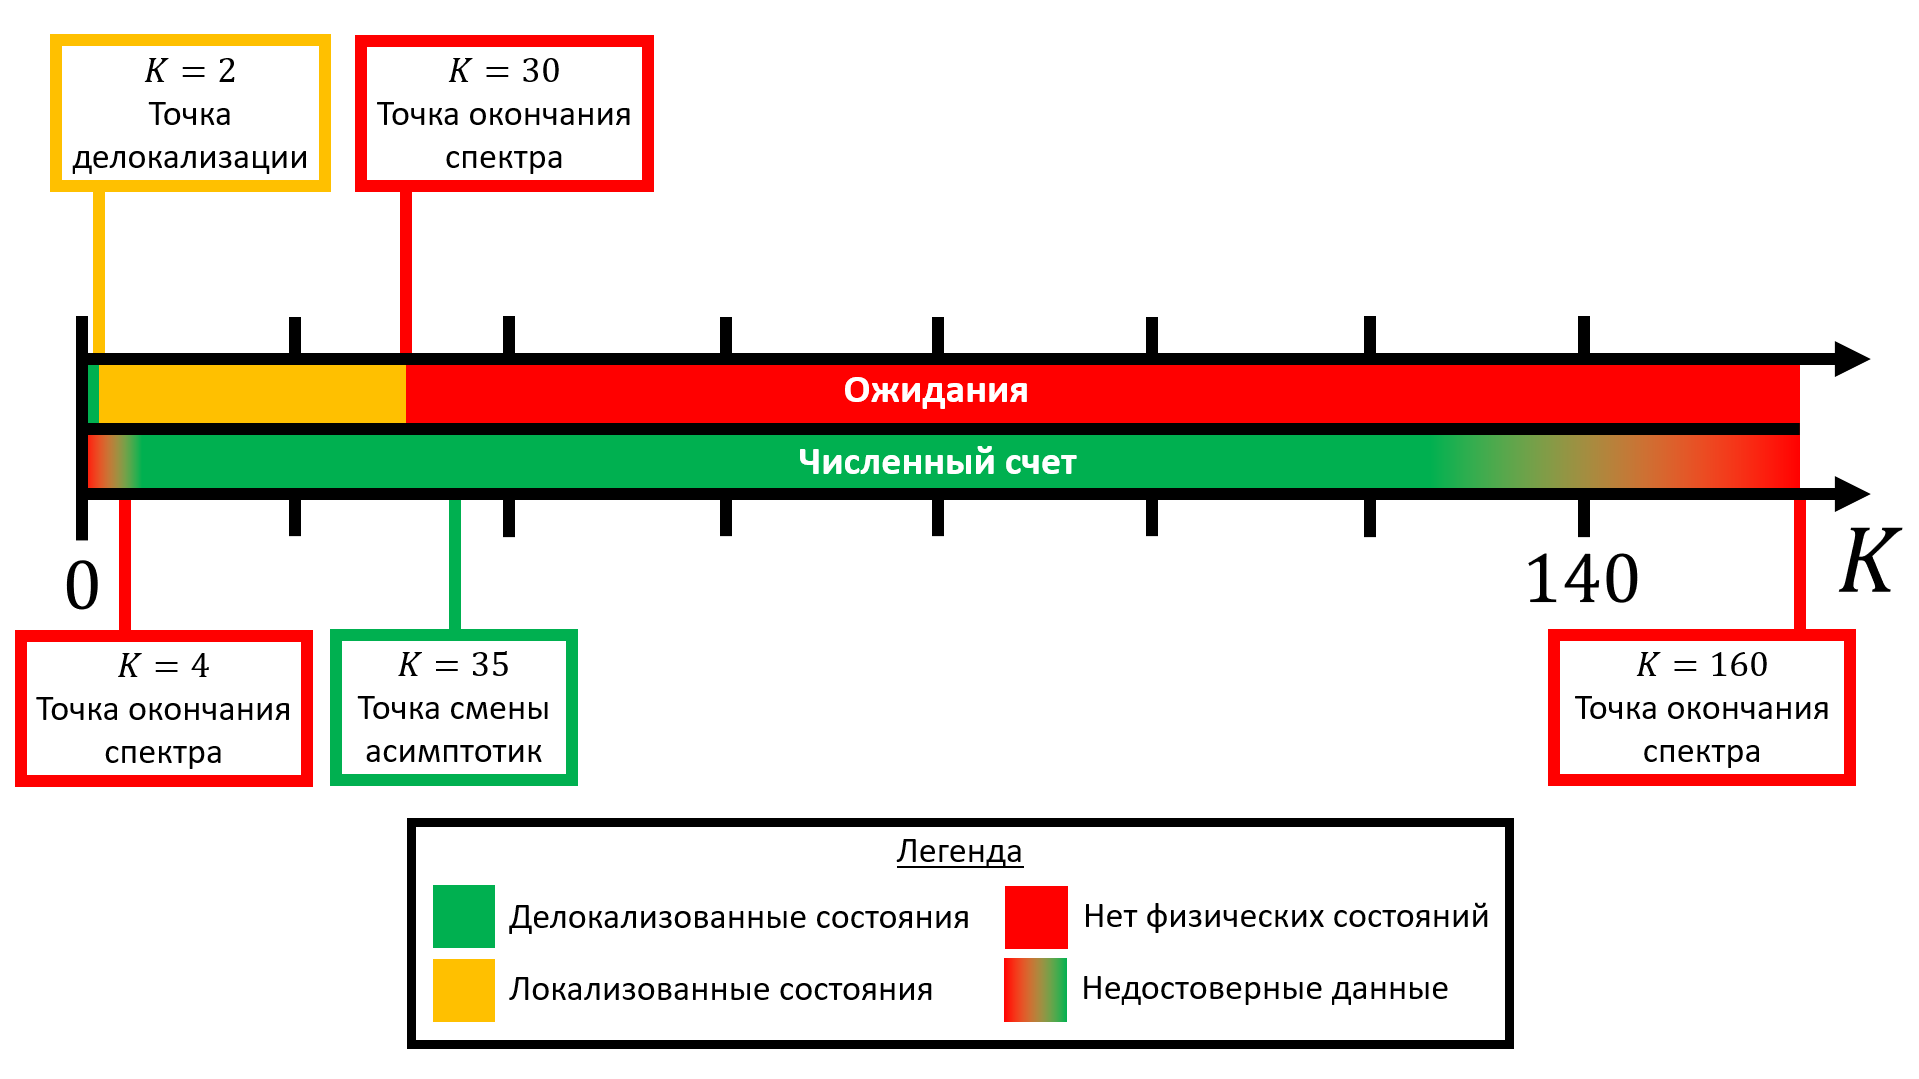
\includegraphics[width=0.9\textwidth]{Phase_diagram.png}
	\caption{Фазовая диаграмма на основании результатов численного счёта. Для сравнения над ней также приведена ожидаемая фазовая диаграмма по статье \cite{FI_microwave}. На диаграмме разным цветом качественно различные диапазоны значений параметров. Градиентной заливкой обозначены неточности в границах зон, вызванные конечной разрешающей способностью численного счёта. На рисунке также отмечены все характерные точки.}
\end{figure}

Чтобы кратко резюмировать качественные сведения, полученные из результатов численного счёта, предлагается фазовая диаграмма, изображённая на Рис. \ref{fig:Phase_diagram}. Для сравнения также приведена диаграмма, предсказанная в \cite{FI_microwave}. Главным выводом, очевидным исходя из этой диаграммы, является то, что эти предсказания \textit{совершенно не подтвердились}. Далее мы разберёмся в причинах этих расхождений.


\section{Основные выводы из результатов}
Подведём итоги увиденного в данных численного счёта: попробуем объяснить расхождения с теоретическими предсказаниями и дадим интерпретацию результата в терминах исходной задачи поиска низкоэнергетических возбуждений.


\subsection{Взгляд с точки зрения задачи Андерсона}
Прежде всего, дадим теоретические пояснения различий между реальной картиной и предсказаниями статья \cite{FI_microwave}. Объяснение можно извлечь из ранее упомянутого в \autoref{Numer} совпадения уравнений популяционной динамики \eqref{eq:Population_dynamics_final_equations} c таковыми для задачи локализации Андерсона на решётке Бете с диагональным беспорядком $\frac{K}{g} \eta^{-1}$ на узле в центре зоны (далее, просто <<задачи Андерсона>>). Авторами статьи \cite{FI_microwave} также неявно было использовано это соответствие, но только в приближённой редакции т. н. Anderson's Upper Limit Condition \cite{AAT}, что и приводит к расхождения с численными данными. Более детальные рассуждения следующие:
\begin{itemize}
	\item Положение точки локализации $K_1$ в работе \cite{FI_microwave} находилось из следующего условия, эквивалентного оценке Anderson's Upper Limit:
	\begin{eqnarray}
		\label{eq:IF_condition}
		\exp \left\{ f(x) \right\} \equiv K \int \limits_0^1 d\xi \left[ \frac{g}{K} \eta\left(\omega|\xi\right)^{-1} \right]^{2 x}= 1, \frac{\partial f}{\partial x} = 0
	\end{eqnarray}
	С точки зрения буквально задачи Андерсона, решение этого уравнения эквивалентно наличию распределения плотности состояний со степенным поведением с показателем $x + 1$. Приближение же состоит в том, что при выводе происходит пренебрежении статистикой действительной части функции Грина. Однако, более аккуратный анализ точного интегрального уравнения, возникающего на распределение плотности, позволяет показать \cite{AAT}, что строго в точке перехода величина $x$ \textit{всегда равна критическому значению $x_c = 1/2$}. С учётом этой поправки, уравнение даёт правильный ответ в лидирующем порядке по $1/K$. Однако, с этой точностью при подстановке правильного значения $x = 1/2$ сам параметр $K$ \textit{из уравнения полностью исчезает}, что означает отсутствие какого-либо перехода по параметру $K$ c точностью $1/K$. Заметим, что описанная согласно \cite{AAT} картина полностью подтверждается численным счётом, в том числе количественно:
	\begin{itemize}
		\item состояния делокализованы при всех $K$, при которых они вообще наблюдаются.  
		\item Однако, если подставить в уравнение \eqref{eq:IF_condition} правильное значение $x = 1/2$, то при $\omega = 0$ мы получим \textit{буквально уравнение самосогласования теории БКШ \eqref{eq:Order_parameter_self_consitency_BCS_limit}}, которое в нашей модели всегда выполнено. Следовательно, наша модель \textit{всегда} находится близко к порогу локализации. Это прекрасно согласуется с наблюдаемой картиной: мы всегда наблюдаем критическое значение показателя степени у распределения плотности состояний и значительное отличие между средним и типичным.
		\item В связи с этим фактом также существует вероятность, что в областях, которые не удалось разрешить численным счётом, состояния локализуются перед тем, как исчезнуть. Это предположение не лишено смысла, так как при ненулевом беспорядке в стандартной задаче Андерсона на дереве между краем спектра и точкой локализации есть область конечного размера по энергии с локализованными состояниями \cite{Biroli_2010}.
	\end{itemize}
	\item Значение точки исчезновения состояний $K_2$ ранее находилось с помощью того же приближенного уравнения \eqref{eq:IF_condition} в предположении, что состояния локализованы перед тем, как пропадут. Однако, как мы убедились, эти предпосылки изначально неверны, а потому положение края спектра для данной модели также найдено неверно. 
\end{itemize}

Развитая на данный момент теория задачи Андерсона позволяет сделать ещё ряд качественных и количественных заключений, важных для понимания полученных результатов. Далее мы будем активно опираться на статью \cite{Biroli_2010}.
\begin{itemize}	
	\item \textit{С математической строгостью} можно найти точное значение края непрерывного спектра (того, что даёт конечный вклад в плотность состояний в термодинамическом пределе). Далее мы приведём рассуждения физического уровня строгости, которые могут быть аккуратно доказаны. Край спектра задачи Андерсона определяется исключительно случаями <<резонансного>> поведения беспорядка, когда в образце образуется большая область с одинаковым значением случайных величин, задающих беспорядок. Такой области соответствует значение энергии
	\begin{equation}
		\label{eq:Edge_energy_Anderson_model}
		E_* = 2 \sqrt{K} - \frac{K}{g} \frac{1}{\eta_{min}} = 2 \sqrt{K} - \frac{\Delta K}{g}
	\end{equation}
	где первое слагаемое -- максимальное собственно значение непрерывного спектра оператора Лапласа на решётке Бете, а второе слагаемое -- максимальное значение беспорядка. Нас интересует собственное число $E = 0$, а потому край спектра определяется условием $E_* = 0$, откуда получаем:
	\begin{equation}
		\label{eq:Edge_of_the_spectrum_in_Anderson_model}
		K_* = \left( \frac{2 g}{\Delta} \right)^2 = g^2 \exp\left\{ \frac{2}{g} \right\}
	\end{equation}
	\item Однако, при использованных в численных симуляциях значениях $g$ край спектра находится в точке $K_* \approx 1.4 \cdot 10^4$. Возникает резонный вопрос: почему же полученная нами оценка на положение края спектра $K \sim 160$ даже по порядку величины неверна? На сей раз, строгого ответа у автора данной работы не имеется, но возможно дать убедительное полуколичественное рассуждение: как уже упоминалось, край спектра находится в точке \eqref{eq:Edge_of_the_spectrum_in_Anderson_model} за счёт областей, в которых величины беспорядка все приняли близкие значения. Вклад в плотность состояний, соответствующую таким областям, можно оценить на основе вероятности такого совпадения значений. Следуя методике, предложенной в \cite{Biroli_2010}, для нашей системы получаем, что зависимости плотности состояний от расстояния до края спектра по энергии $\delta E$ есть
	\begin{equation}
		\label{eq:DoS_near_edge_estimation}
		\rho(\delta E) \sim \exp \left\{ -\frac{K+1}{K} K^{\pi K^{1/4} / \delta E^{1/2} } \ln \frac{1}{ \sqrt{2 \Delta \delta E} } \right\}
	\end{equation}
	Далее, поскольку в терминах задачи Андерсона мы интересуемся плотностью состояний на энергии $E = 0$, то $\delta E \equiv E_*$ -- некоторая плавная функция $K$. С другой стороны, функция \eqref{eq:DoS_near_edge_estimation} является \textit{очень резкой}, так что при приближении к краю спектра эта плотность состояний очень быстро принимает микроскопические значения. На практике полученная величина \eqref{eq:DoS_near_edge_estimation} является оценкой снизу, в то время как реальная плотность состояний обеспечивается и другими механизмами кроме вышеописанной схемы <<резонансов>>. Поэтому в момент, когда все прочие механизмы теряют свою эффективность, плотность состояний практически мгновенно принимает значения, не отличимые от нуля никакими практическими методами, в том числе и численными. Именно этот факт и отражает найденная нами точка $K \sim 160$.
	\item Наконец, ещё одно важное следствие приведённых рассуждений состоит в том, если описанное поведение в духе уравнения \eqref{eq:DoS_near_edge_estimation} действительно имеет место, то край спектра задачи \textit{не имеет никакого физического значения}: если им задаётся какая-то реальная физика, то столь малая плотность состояний не обнаружима никакими доступными экспериментальными методами.
\end{itemize}


\subsection{Интерпретация в терминах исходной задачи низкоэнергетических возбуждений}
Наконец, дадим некоторые комментарии по поводу значения полученных результатов для исходной задачи описания низкоэнергетических возбуждений в сверхпроводнике. Изначально она ставилась в терминах спектральных свойств некоторого, вообще говоря, нелокального оператора \eqref{eq:Investigated_linear_operator}, после чего было показано, что конечная плотность состояний и свойства локализации собственных мод в этой задаче связаны некоторой гладкой ненулевой функцией с таковыми для локального оператора \eqref{eq:Local_operator_definition} в собственном значении $1$. На основании этих рассуждений и полученных нами результатов можно сделать главные на данный момент выводы по проделанной работе: 
\begin{itemize}
	\item поскольку плотность состояний локального оператора вблизи края спектра ведёт себя негладки образом, то такого же неаналитического поведения следует ожидать и от плотности возбуждений. А значит, и для исходного оператора \eqref{eq:Investigated_linear_operator} вопрос края спектра также не имеет глубокого смысла, поскольку такая ничтожная плотность состояний не может быть обнаружена никакими физическими опытами.
	\item Поскольку свойства локализации у двух задач совпадают, а для локальной задачи наши результаты состоят в том, что моды всё время делокализованы, то тоже самое верно и для возбуждений в рамках изучаемой модели. В частности, результаты потенциально означают диссипативное поведение во всей области параметров, что уже прямо противоречит экспериментальной картине.
\end{itemize}
Резюмируя, \textit{построенная модель не отображает реальной физики низкоэнергетических возбуждений}. Укажем несколько возможных причин и следующие из них пути улучшения построенной модели.
\begin{itemize}	
	\item Главной причиной автор работы считает приближение, связанное с игнорированием распределения параметра порядка по узлам системы. Как мы видели в обсуждении полученных зависимостей, локализация в данной задаче не наступает с точностью $1/K$. Единственным эффектом порядка $1/K$, который был выкинут при построении модели, являются отклонения параметра порядка от своего среднеполевого значения \eqref{eq:Order_parameter_BCS_limit}. Напомним также, что это приближении лишает локальный оператор \eqref{eq:Local_operator_definition} собственного состояния с собственным числом $1$, являющегося Голдстоуновским возбуждением нарушенной фазовой $U(1)$-симметрии. 
	
	\item Далее, важно упомянуть, что строго говоря, в \autoref{Theor} был установлен лишь факт совпадения положения характерных точек обеих моделей. При этом никаких утверждений касательно количественной связи плотности состояний в двух моделях не делалось. Поэтому в общем случае необходимо также исследовать, как связаны количественные характеристики двух моделей.ы
\end{itemize}


\subsection{Планы дальнейших исследований}
Как следует из обсуждения выше, дальнейшее направление развития построенной модели следующее:
\begin{itemize}
	\item изучить более подробно решение уравнения самосогласования \eqref{eq:Order_paramter_self_consistency} в следующем порядке по $1/K$ и, в частности, исследовать возникающее совокупное распределение полей $\eta_i$, в которые входит значение параметра порядка на узле, тем самым делая величины $\eta_i$ также коррелированными.
	
	\item По итогам исследования структуры решения уравнения самосогласования необходимо поставить задачу, учитывающую найденные корреляции и пригодную для численного и/или аналитического исследования.
	
	\item С другой стороны, вполне вероятно, потребуется модификация существующей численной процедуры, учитывающая корреляции на узлах. В частности, метод популяционной динамики в исходной редакции не приспособлен к исследованию коррелированного беспорядка.
	
	\item Отдельным пунктом можно упомянуть исследования степени количественной схожести спектральных задач для операторов \eqref{eq:Investigated_linear_operator} и учитывающего корреляции варианта оператора \eqref{eq:Local_operator_definition}, так как на данный момент продемонстрирована лишь соответствие их качественного поведения.
\end{itemize}
